%!TEX root = ../physical-olympics-2.tex
\chapter{运动学}

\section{时空与物质}

物理学,\,从刚开始成为实验性的科学的伽利略时期开始,\,到近半个世纪年来理论物理学家对额外维度的探讨,\,都给予了\emph{时空}(spacetime)最核心的地位.\,牛顿的理论,\,分析力学,\,经典场论,\,相对论这些理论最基本的图像都是时空与\emph{物质}(matter)的分立性.\,时空是装备了一个能体现出物理物理意义的\emph{度量}(metric)的3+1维对象\footnote{数学上有一套严格的说法,\,把这种连续,\,光滑的四维对象称为\emph{伪黎曼流形}(pseudo-Riemannian manifold).}.\,而物质是在每个时空点处的某种结构.\,下面会分别介绍不同物质体系的描述方法.\,在这之前我们来看看不同的时空观:

\subsection{时空观,\,坐标系}
牛顿力学理论体系基于\emph{伽利略时空观}(Galilean spacetime picture),\,也就是\emph{绝对时空观}(absolute spacetime picture).\,在这里空间是三维的平直空间.\,设想一个人站在该空间的某个空间点,\,他的胸前,\,头顶和右手平举的三个方向就是相互垂直的方向.\,如果以自己的臂长为标准长度,\,他能够定义空间中每两个点之间的空间间隔.\,事实上,\,这个人能够以一种正确的方式为每个空间点定义一个坐标,\,那么所有三维空间点的集合与任意两个点之间的距离为:
\[A(x,y,z)\in\mathbb{R}^3 \quad;\quad x,y,z\in\mathbb{R}\]
\[A(x_1,y_1,z_1)\;,\;B(x_2,y_2,z_2)\;:\;l^2=\overline{AB}^2=(x_1-x_2)^2+(y_1-y_2)^2+(z_1-z_2)^2\]

因为空间不同于时间,\,我们为以上数字赋予特殊的物理含义,\,也就是加上\emph{量纲}(dimension).\,如果两点坐标为$(0,0,0)$和$(1,1,1)$,\,那么$l=\sqrt{3}{\rm m}$,\,而不是$l=\sqrt{3}$.\,其单位${\rm m}$一方面表示了这个物理量的属性,\,另一方面指定了某个实际物理体系确定下来的固有长度大小.\,现行的(2018年1月1日,\,下文同)国际单位制对$1{\rm m}$的定义如下\footnote{一方面,\,它依赖于狭义相对论的正确性,\,目前极少理论物理工作者会质疑它.\,另一方面,\,应该要先定义下文的1s,\,再来定义1m.}:
\begin{verse}
1m是光在1/299792458\,s内在真空中行进的距离.
\end{verse}


这就是我们的\emph{三维平直空间}(3-dimensional flat space).\,注意空间点具有物理实际意义,\,它可以脱离坐标系而单独存在.\,事实上坐标系的原点可以建立在空间中的任意点处,\,朝向也可以是任意方向,\,两个空间点之间的距离$l$不会依赖于坐标系的选取,\,但两个点的坐标会因坐标系不同而改变.\,如果我们选取的坐标系总是下述使得两个相距很近的点之间的微元距离公式成立:
\[\ud l^2=\ud x^2+\ud y^2+\ud z^2\]


那么建立的坐标系就是一个\emph{笛卡尔坐标系}(Cartesian coordinate system),\,即\emph{空间直角坐标系}(3D orthogonal coordinate system).\,但是以空间直角坐标系为基础,\,我们又经常建立\emph{球坐标}(spherical coordinate)和\emph{柱坐标}(cylindrical coordinate)系统.\,通常取$x$轴为\emph{幅轴}(azimuth axis),\,点在$x-y$平面上的投影与原点的连线相对$x$轴转过的角度为$\varphi$,\,即\emph{幅角}(azimuth angle).\,而$z$轴为\emph{极轴}(polar axis),\,而点与原点连线与极轴的夹角$\theta$为\emph{极角}(polar angle).\,天文观测用球坐标就很方便,\,它是以描述的空间点到原点之间的距离$r$,\,也称\emph{矢径}(radius),\,和两个描述角位置的极角幅角来构成三个坐标$(r,\theta,\varphi)$的.\,而理论物理里也常用到的柱坐标是以$(\rho,\varphi,z)$为描述空间点的坐标,\,$\rho$是空间点到$z$轴的距离.

\begin{wrapfigure}[14]{o}[-10pt]{7cm}
\vspace{-0.4cm}
\centering
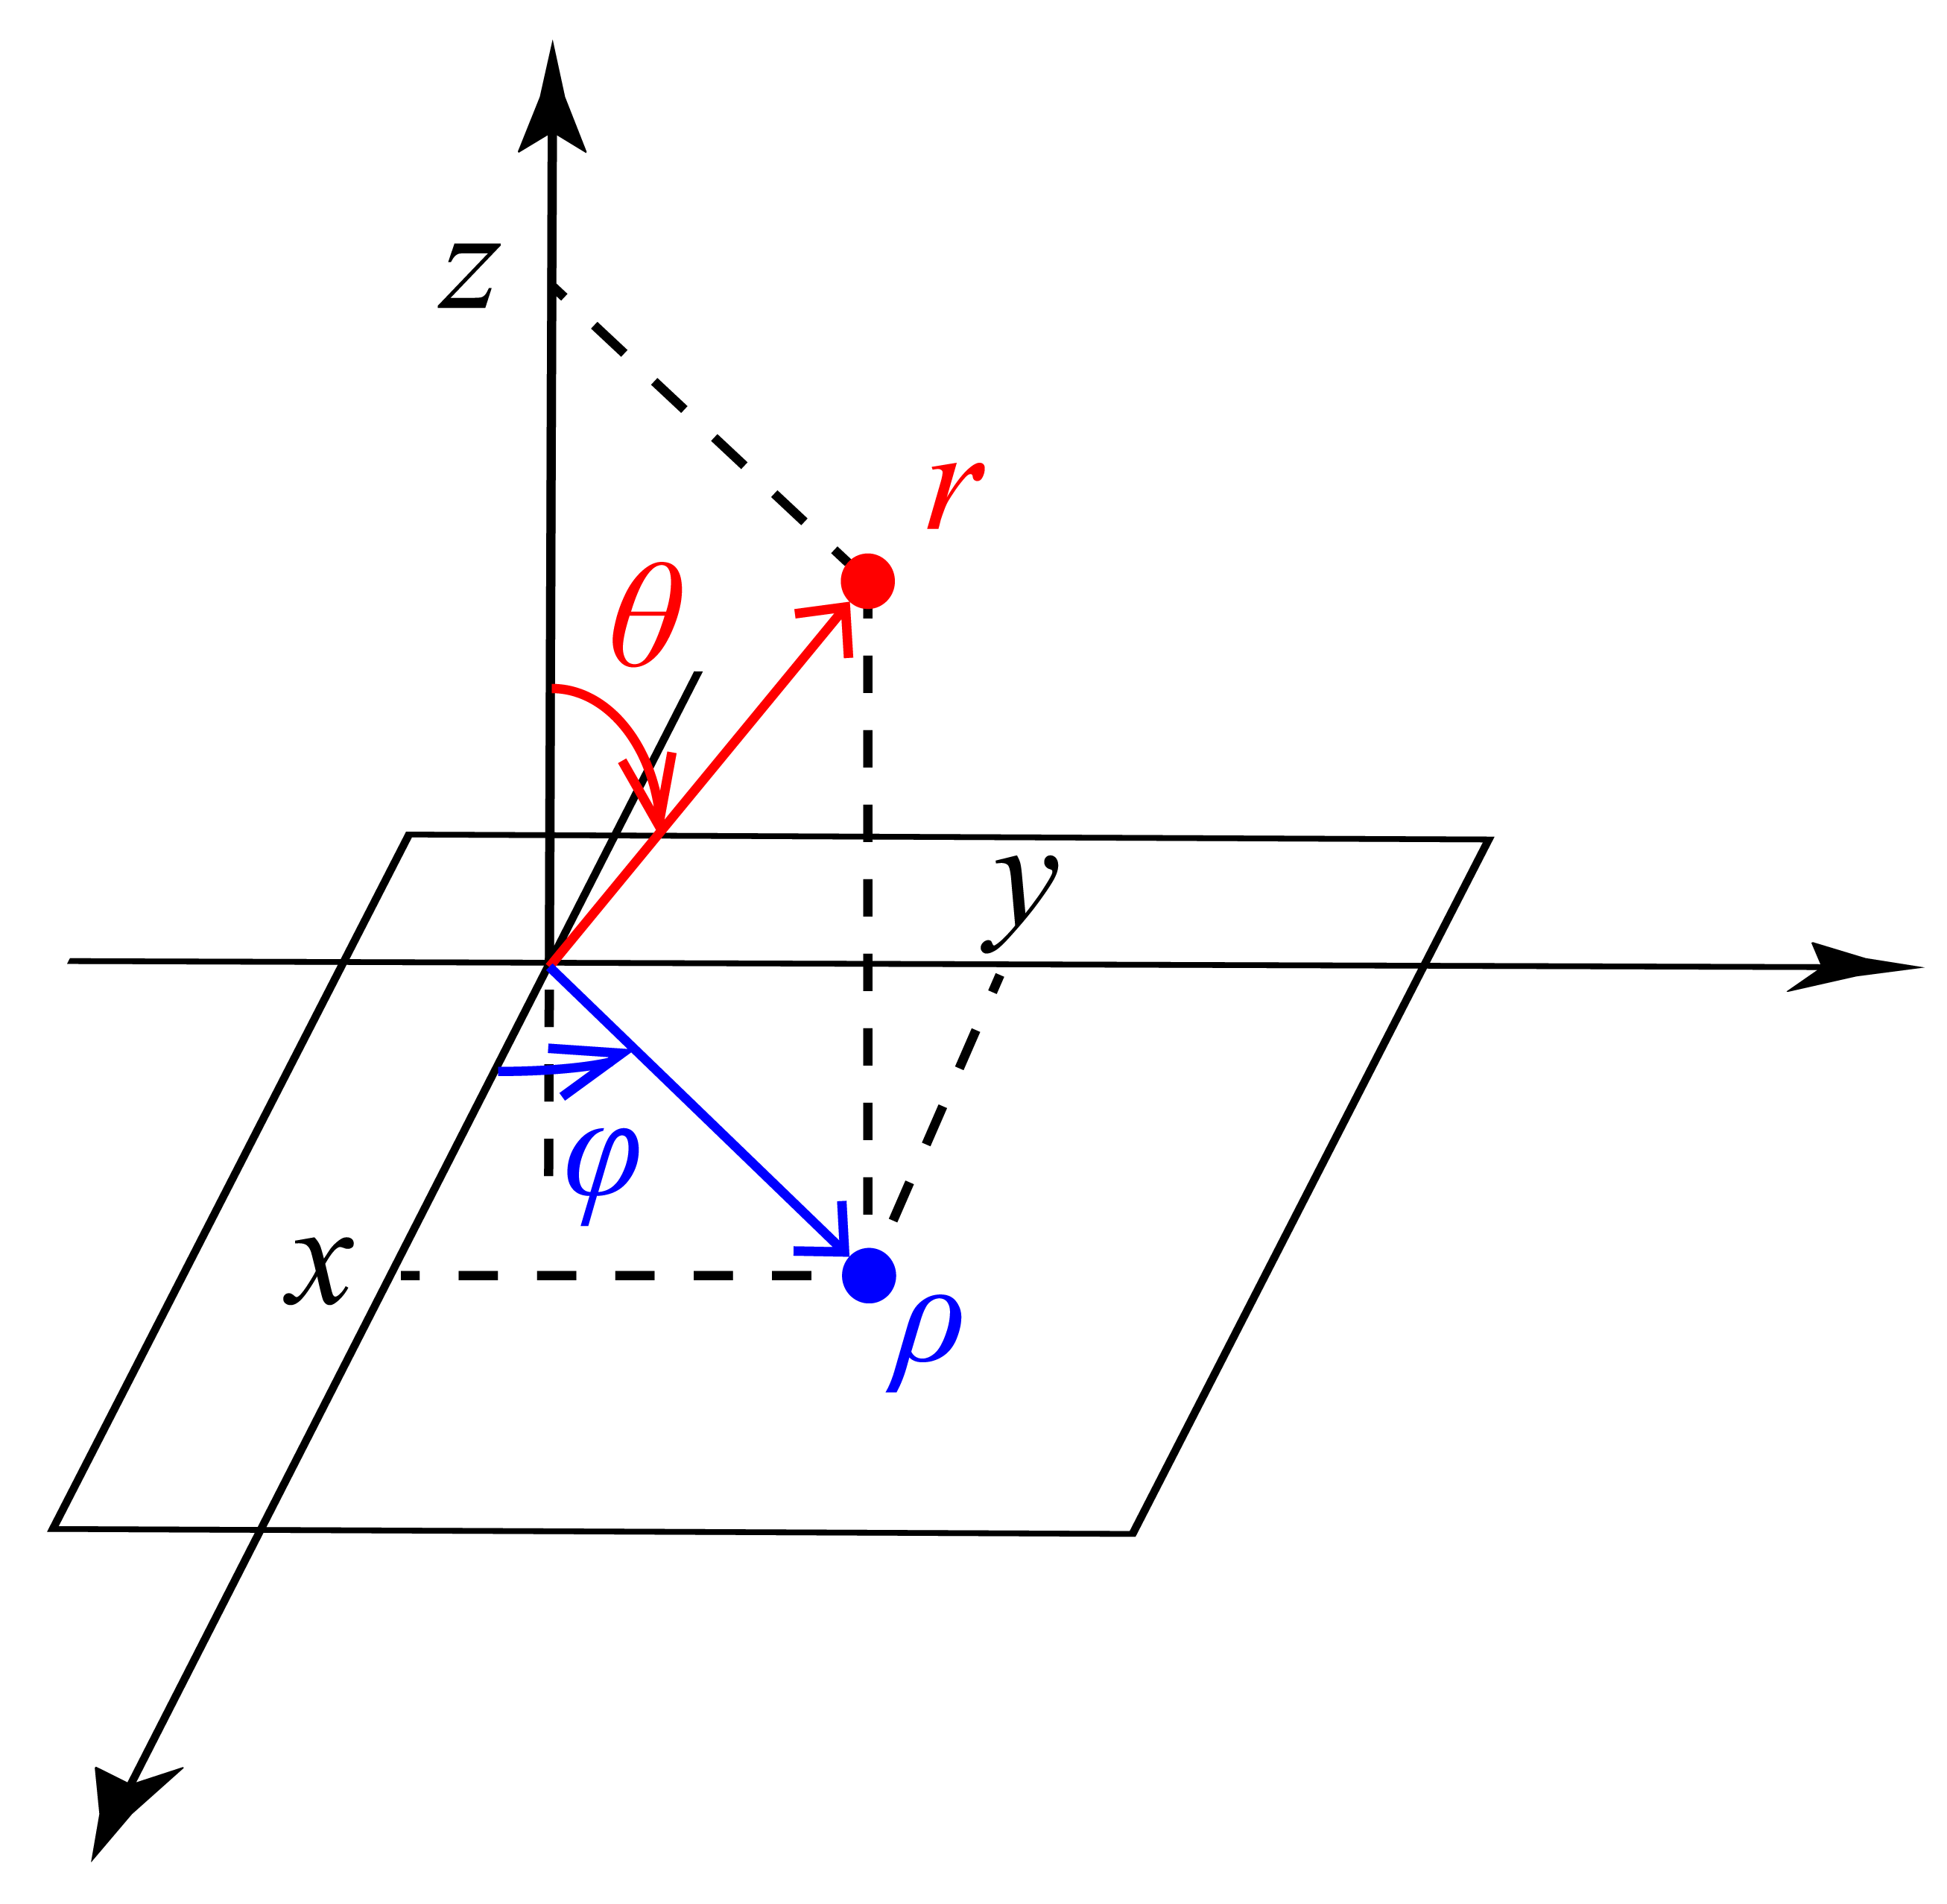
\includegraphics[width=7cm]{image/6-1-1.png}
\caption{三种坐标}
\end{wrapfigure}
需要注意,\,我们对以上$\theta,\,\varphi$角度定义比较微妙,\,$\theta$一般限制其在$[0,\pi]$范围内,\,在端点$\theta=0,\,\pi$处$\varphi$的不同取值代表同一个空间点.\,但$\varphi$的取值我们不加以任何限制,\,也就是原则上$\varphi\in\mathbb{R}$.\,而任意$\varphi$相差$2n\pi$的坐标实际上代表同一个空间点.\,这么做是因为我们最好不要用静态的几何观点去看待角度这一概念.\,而是用运动,\,变换的观点去看待角度.\,作为连续的运动的点的幅角变化也应是连续的,\,为了使点绕$z$轴一圈后幅角不至于突然改变,\,就必须默认每一点的幅角可以有多种取值,\,在具体的运动中应该灵活选择其具体取值大小.

之后经常会说到各种对称性,\,在本系列教材中我们采取如下说法:\,\emph{球对称}(spherical symmetric)仅仅代表某个函数$f(r,\theta,\varphi)$与$\varphi$无关.\,而\emph{柱对称}(cylindrical symmetric)代表的是$f(\rho,\varphi,z)$与$z$无关.\,与$\varphi$和$\theta$都无关的$f(r,\theta,\varphi)=f(r,\forall\theta,\forall\varphi)$被称为\emph{各向同性}(isotropic).\,最后\emph{中心对称}(centrosymmetric)是一个很弱的对称性,\,它仅仅代表函数在\emph{中心反演}(space inversion)下的对称性:
\[f(x,y,z)=f(-x,-y,-z)\]

绝对时空观中的时间则是一种完全与空间独立的属性.\,实际上,\,每一个空间点处的人都能感受到时间的流逝.\,十分抽象的把这些不同的时刻画在一根时间轴上,\,便是一维的时间坐标:
\[A(t)\in\mathbb{R} \quad;\quad t\in\mathbb{R}\]

而时空又是两个独立的概念.\,任意一个坐标点处都有时间轴,\,而任意一个时刻都有一个三维空间切片.\,事实上,\,我们的时空是一个3+1维的结构,\,合理地选取坐标后,\,实际上可以把时空结构写成四维坐标:
\[A(x,y,z,t)\in\mathbb{R}^4 \quad;\quad x,y,z,t\in\mathbb{R}\]

而对于任意两个时空点,\,存在绝对的时间,\,也就是可以找到两个事件的绝对时间差:
\[\tau=|t_2-t_1|\]

但空间距离却具有相对性.\,我们要求在同一时刻的同一空间切片上定义空间的度量:
\[t_1=t_2:\quad l=\sqrt{(x_1-x_2)^2+(y_1-y_2)^2+(z_1-z_2)^2}\]

不同时刻的空间,\,被线性地组织在一起,\,保证每一刻都平直的空间既不会随时间膨胀收缩,\,也不会旋转加速.\,这种时空结构被叫做\emph{牛顿-嘉当几何}(Newton-Cartan geometry)\footnote{用更为严格的语言来说,\,我们需要一个装备了一阶形式``钟''$c_\nu$和二阶逆变半正定对称张量类空间度规$s^{\mu\nu}$的四维微分流形$\mathscr{M}$:
\[\mathscr{M}:\quad s^{\mu\nu}c_{\nu}=0\]}.

时间是一个新的量纲,\,其国际单位制对$1{\rm s}$的定义为:
\begin{verse}
1s是铯-133原子基态的两个超精细能级之间跃迁所对应的辐射周期时长的9192631770倍.
\end{verse}

牛顿-嘉当几何的显著特点是物理量的定义没有所谓的\emph{协变性}(covariance).\,固然,\,在三维空间坐标框架的旋转下,\,任何物理过程中的事件所发生的位置坐标发生旋转变换,\,而几乎所有标量(比如质量,\,能量)都不变,\,几乎所有矢量(比如动量,\,角动量)都按照类似坐标变换的法则发生变换.\,但是,\,对于更普遍的一列\emph{伽利略变换}(Galilean transformation),\,也就是相对匀速运动的参考系之间的变换,\,时空坐标的形式却不能简单地推广到能量动量角动量上.

不同于绝对时空观中时间与空间成为相互独立的量纲的特点,\,狭义相对论改变了对基本物理量的看法.\,狭义相对论把时空看成为可以相互转化的不可分割的新的3+1维整体,\,同时性已然破缺.\,两个时空点之间无法定义绝对的时间间隔.\,在\emph{相对论时空观}(relativistic spacetime picture)下,\,时间和空间可以用同一把尺子去丈量:\,这是由于光速的不变性:
\[c=299792458{\rm m/s}\]

而量出来的长度叫做\emph{时空间隔}(spacetime interval):
\[\ud s^2=c^2\ud t^2-\ud x^2-\ud y^2-\ud z^2\]

这赋予时空以截然不同的结构,\,最关键的一点是,\,时间的绝对性被取消了,\,不同事件发生时间先后的比较不总是可行,\,相对论的有限速度因果律在这里取代了经典观点的时序因果律.\,我们将在本书最后介绍相对论理论.


\subsection{物质}

时空是物理过程发生的舞台.\,那么将物质引入后舞台上所演出的便是\emph{事件}(event).\,事件这个物理概念由这样的数学工具来描述:\,它的第一个要素自然是时空坐标$(\bs{r},t)$,\,是事件在时空上的外化.\,第二个要素是事件内禀的属性.\,它取决于所引入的物质种类,\,还取决于我们所关心问题的层次.\,一般用标量,\,矢量,\,乃至张量这样的数学工具来描述它.\,举例,\,电磁场物质在经典物理中用电场磁场来描述,\,但在\emph{量子力学}(quantum mechanics,\, QM)中这不够了,\,需要用矢势和标势来描述才是完整的.\,在更深的\emph{量子场论}(quantum field theory)中甚至这也是不够的.\,还需要量子化为光子才合适.\,又比如,\,电子这个很有意思的现象,\,最简单的模型是质点模型,\,内禀的属性是质量,\,动量与能量\footnote{不要认为动量能量不是内禀的而是由时空运动所决定的,\,读者可以思考在水中一个气泡的上升,\,它为体系带来的动量方向如何?}.\,然而与电磁场的经典相互作用强度告诉我们还有一项内禀属性叫做电荷量.\,近代人们惊奇地发现原来电子还固有磁矩,\,也就是电子的自旋.\,最后狄拉克等人发展出\emph{量子电动力学}(quantum electrodynamics,\,QED),\,统一地用一个四分量的旋量波函数和它的方程中的若干参数来完整地描述所有发现的电子内禀属性.

\vspace{0.5cm}
\emph{经典物理学}\footnote{本书的经典物理学指牛顿力学,\,分析力学,\,经典电磁学,\,经典统计力学与狭义相对论的范畴.}(classical physics)中涉及到的物质主要有:

\vspace{0.2cm}
{\bf 1.\,质点(point mass,\,particle)}

不得不承认质点是牛顿力学的根基,\,一切可观的结论的出发点.\,质点所对应的事件集合为时空中的一条\emph{世界线}(world line).\,每一个时间仅仅有可能只有一个事件发生.\,实际上质点的运动用\emph{运动学方程}(kinematic equation)来描述:
\[\bs{r}=\bs{r}(t)=\left(x(t),y(t),z(t)\right)\]

而\emph{质量}(mass)是质点必要的内禀属性.\,它将作为参数出现在下一节介绍的动力学方程中.\,它反应物质受到同样大小的相互作用运动状态改变的难易程度.\,国际单位制对$1\rm kg$的定义如下:

\begin{verse}
1kg是保存在法国巴黎布勒特伊宫的国际计量局实验室的约47立方厘米立式铂铱合金小圆柱的质量.\,当然,\,处于实用考虑,\,也是很多它的官方复制体的质量.
\end{verse}

这个定义从1889年至今已经有一百多年了,\,历史远长于其他六个国际基本单位.\,2018年末将有望修改这一古老的定义方式,\,新的定义\footnote{一方面,\,它依赖于狭义相对论和量子力学的正确性,\,目前极少理论物理工作者会质疑它.\,另一方面,\,应该要先定义上文的1s和1m,\,再来定义1kg.}为:

\begin{verse}
1kg被这样定义:\,取普朗克常数的固定数值在单位$\rm kg\cdot m^2\cdot s^{-1}$下为$\rm 6.62607015\times 10^{-34}$.
\end{verse}

长度,\,时间和质量为三大力学量纲,\,量纲是物理量的属性,\,物理量的表示方法为数值加单位,\,每个量纲有自己独特的一套单位,\,不同单位间差一个纯数的倍率.\,在物理量的加减时量纲必须相同而且结果保持量纲不变.\,但不同量纲物理量可以进行乘除而生成新的量纲.\,除了简单的加减乘除的以上规则以外,\,其他特殊函数必须只能作用在无量纲的纯数上.\,这叫做\emph{量纲法则}(dimensional rules).

\vspace{0.2cm}
{\bf 2.\,质点系(particle system)}

质点系是对质点的一种自然扩展.\,讨论质点的运动时质点受到的相互作用来自何方?\,在牛顿力学的框架下必然来自施力物体.\,故把两个质点作为整个体系讨论,\,把相互作用区分为内力与外力而推广之前的结论,\,在这个过程中我们能体会到哪些结论是一脉相承的普遍规律而哪些需要重新审视与修改.\,从原理上质点系不过是多个质点同时存在的情况而已.\,而经典统计力学是这种观点的提炼与延伸,\,它着眼于一个宏观大分子数的体系的长时间平均下的行为,\,理论上常常结合概率论的做法,\,对等概率的体系代表点构成的系综做平均.\,从中提取统计力学下不平凡的物理量.

\vspace{0.2cm}
{\bf 3.\,连续介质(continuous media)}

一方面,\,连续介质是从纯粹的理论过渡到实际问题的至关重要一步.\,另一方面,\,在处理连续介质的问题中形成了场论,\,它作为了一种与质点截然不同的物理图像形成了自己的一整套理论.\,更重要的,\,量子场论认为由于不确定原理,\,质点与世界线的观点实际上是作为场的传播的一种近似.\,也就是说,\,场论相比质点的力学更具有兼容性和普适性.\,对于简单的连续介质,\,内禀的属性由每一个点处的质量密度$\rho$和速度$\bs{v}$描述,\,这实际上形成了一个标量场和矢量场:
\[\rho=\rho(\bs{r},t) \quad;\quad \bs{v}=\bs{v}(\bs{r},t)\]

而动力学方程的列法又强烈依赖于介质内的相互作用.\,于是这个大的问题又分出很有代表性的弹性力学和流体力学,\,还有介于两者之间的粘弹性塑性模型等等.\,还有从热力学平衡态出发考虑的近平衡态统计力学方法.

\vspace{0.2cm}
{\bf 4.\,场(field)}

\begin{wrapfigure}[16]{o}[-10pt]{7cm}
\vspace{-0.4cm}
\centering
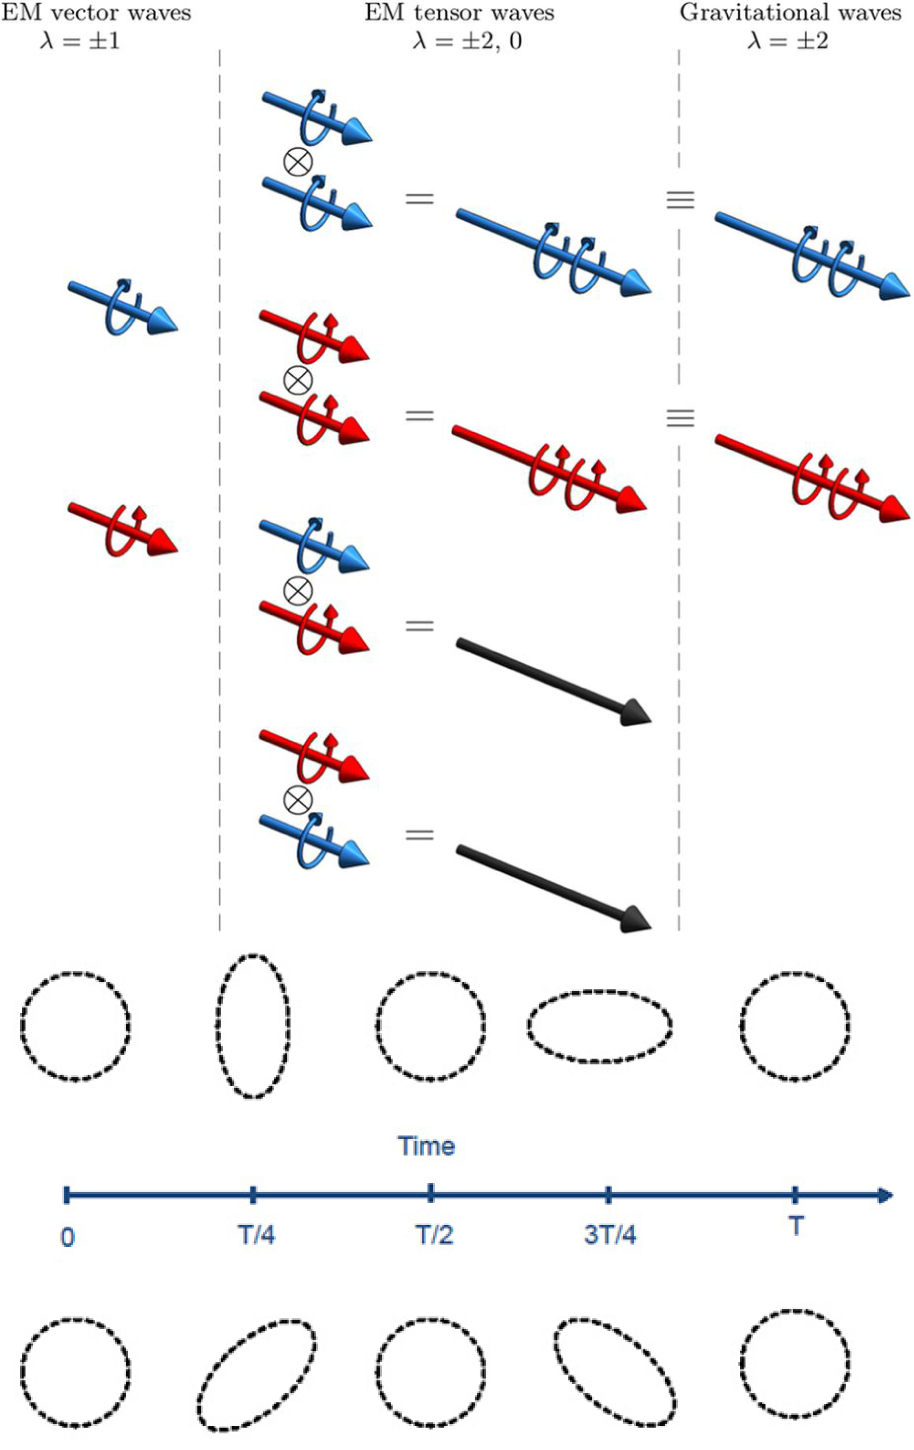
\includegraphics[width=5cm]{image/6-1-2.png}
\caption{引力波与电磁波的区别}
\end{wrapfigure}
关于场的理解历史上经历了两个过程.\,第一个阶段是正如上面的连续介质的做法,\,场是作为某种事先已经被研究的足够清楚的粒子体系与它们之间的相互作用的描述方法与数学工具.\,而从牛顿时代开始人们就默认了超距作用的存在,\,而场数学工具的第二个作用就是描述电荷之间,\,质量之间的超距作用.\,但是逐渐人们意识到相互作用传播速度的有限性,\,于是场开始变成某种与物质其他耦合的物质而单独存在,\,这就是第二阶段,\,人们意识到了场本身就是一种物质,\,电子与电子之间不能直接相互作用,\,电子改变了真空,\,稳定地与电磁场相互作用而产生库仑场,\,然后在对第二个电子产生相互作用力.\,将场作为某种先验地存在于时空中的物质形式进行描述与研究的学科就叫做\emph{场论}(field theory).\,有哪些可能的场形式?\,场的物理量如何书写?\,场与粒子,\,场与场之间如何相互作用便是场论的研究内容.\,比如说,\,动力学所关心的内容,\,场的质量本身没有定义,\,可以定义的一般是场的定域动量与波矢,\,能量与角频率,\,平面波的色散关系等等.\,的确,\,场论最基本的做法是傅里叶分解,\,它认为平面波是不受任何相互作用时的场的惯性运动方式,\,而任何场的运动,\,每一时刻都可以分解成一系列平面波的叠加.\,就好像任何复杂体系的运动本质上都是质点系的运动,\,而质点的运动每时每刻都可以看出匀速运动那样.


场论根据其描述方法分为标量场论,\,矢量场论,\,张量场论和旋量场论等.\,电磁场论是矢量场论,\,它用四势矢量$(\varphi,\bs{A})$来描述.\,引力场论在广义相对论弱场近似下是张量场论,\,但传播的引力波和电磁波类似只能有两种偏振,\,其模式为$+$型和$\times$型,\,这又是不同于电磁波的.\,在更现代的观点中,\,场是真空的某种激发,\,十分类似于一张二维的拉紧的薄膜,\,没有任何振动时它已经固有能量了,\,场物质反应为膜的各种振动形式.\,而一个石子受到外力而压弯了膜,\,就可以理解为粒子与场之间的相互作用.



\subsection{参考系,\,物理规律与其不变性}

\emph{坐标系}(coordinate system)是一套用来描述时空点位置的坐标系统,\,而\emph{参考系}(reference system)则是下文将引申的一类坐标系的统称.

在伽利略时空观\footnote{本章仅限讨论非相对论,\,相对论见后}下参考系的定义相对简单.\,我们只需要任意指定一个观察者,\,观察者可以在$3+1$维的时空中作任意运动,\,每一个时刻对应一个测量的坐标系统:\,观察者分别以右手边,\,胸前和头顶三个方向建立坐标系,\,坐标系的刻度就是其代表的位置到原点观察者处的空间距离.\,这样便可以表示任意事件的时空坐标.\,而且构成一个三维空间直角坐标系.\,叫做观察者的\emph{固有参考系}(proper reference system).

物理规律的本质是什么?\,在一个特定的参考系中,\,我们进行一些物理量的测量,\,测量得到的值之间在特定的实验条件下会满足特定的关系而不依赖于某些具体的参数,\,一般都是等式.\,这样的普遍成立的等式就可以反映某些物理规律.\,从\emph{动理学}(kinetics)的角度理解,\,体系的演化是\emph{状态}(state)随时间的演化,\,而体系的状态由一组完备的\emph{态参量}(state variable)描述,\,态参量可以包含一些广义坐标$q_\alpha$和他们对时间的导数即广义速度$v_\alpha=\dot{q}_\alpha$.\,而以下\emph{决定论}(determinism)则对物理规律的形式做出了规定:
\begin{quote}
动理学系统:

已知某时刻$t=0$的初态$\{q_\alpha(0),\,\dot{q}_\alpha(0)\}$后,\,应能预言任意将来的状态$\{q_\alpha(t),\,\dot{q}_\alpha(t)\}$.
\end{quote}

事实上,\,不光是将来的状态,\,而且在一般经典物理的框架下,\,过去的状态也是可以被``预言''的.\,这是因为我们进一步要求动理学系统的规律是以下形式的二阶方程:
\[f_i(\ddot{q}_\alpha,\,\dot{q}_\alpha,\,{q}_\alpha,\,t)=0\]

而且广义坐标的个数应该和方程的数目一致,\,方程是至多二阶的.\,微分方程的描述在数学上完全导致了体系彻底的决定性,\,只要知道初始条件便可以往前往后推理所有发生的物理现象\footnote{更有甚者,\,经典物理也难以解释耗散现象,\,在忽略耗散时,\,方程应该还具有平移对称性(不显含t)和时间反演对称性(方程对广义速度是偶函数).\,此时对将来和对过去的预言在广义速度取相反数时是完全对称的,\,而且预言只依赖与时间差不依赖于初始时刻.}.

这一物理学科研究范围内的原理很强大,\,强大到历史上很多物理学家和哲学家都质疑过它的真实性和适用性.\,最著名的莫过于拉普拉斯提出的\emph{拉普拉斯妖}(Laplace's demon)的论点:\,如果存在一个全知的拉普拉斯妖,\,能够知道在某一时刻宇宙中所有原子的精确位置与动量,\,那么任意时刻的状态也能被预言.\,这种决定论观点总是被拿来与\emph{自由意志论}(free will)去归谬,\,如果过去与未来都已经被谱写,\,那么人类所有的行为的意义和动机也就不能被解释.\,这直到今天也是科学与哲学未能获得满意的回答的问题.

但是科学的一个目的就是在于能够对未发生的事情进行预言,\,所以本着对决定论的认可与尊重,\,我们才能继续我们的科学研究.

下一个伽利略相对性原理.
\vspace{5cm}



\section{运动的描述}

\subsection{质点的运动}
质点的运动是复杂的连续体的运动的基础.\,所谓\emph{运动}(motion)就是每一个时间都有一个位置.\,就是说位置是时间的函数:
\[\bs{r}=\bs{r}(t)\]

我们使用实数上的矢量空间和矢量来刻画真实的物理学上的二维或三维空间和其中的点.\,也即:
\[\bs{r}\in\mathbb{R}^2 \;{\rm or}\; \mathbb{R}^3\]

\begin{wrapfigure}[16]{o}[-10pt]{7cm}\label{6-1-3}
\vspace{-0.4cm}
\centering
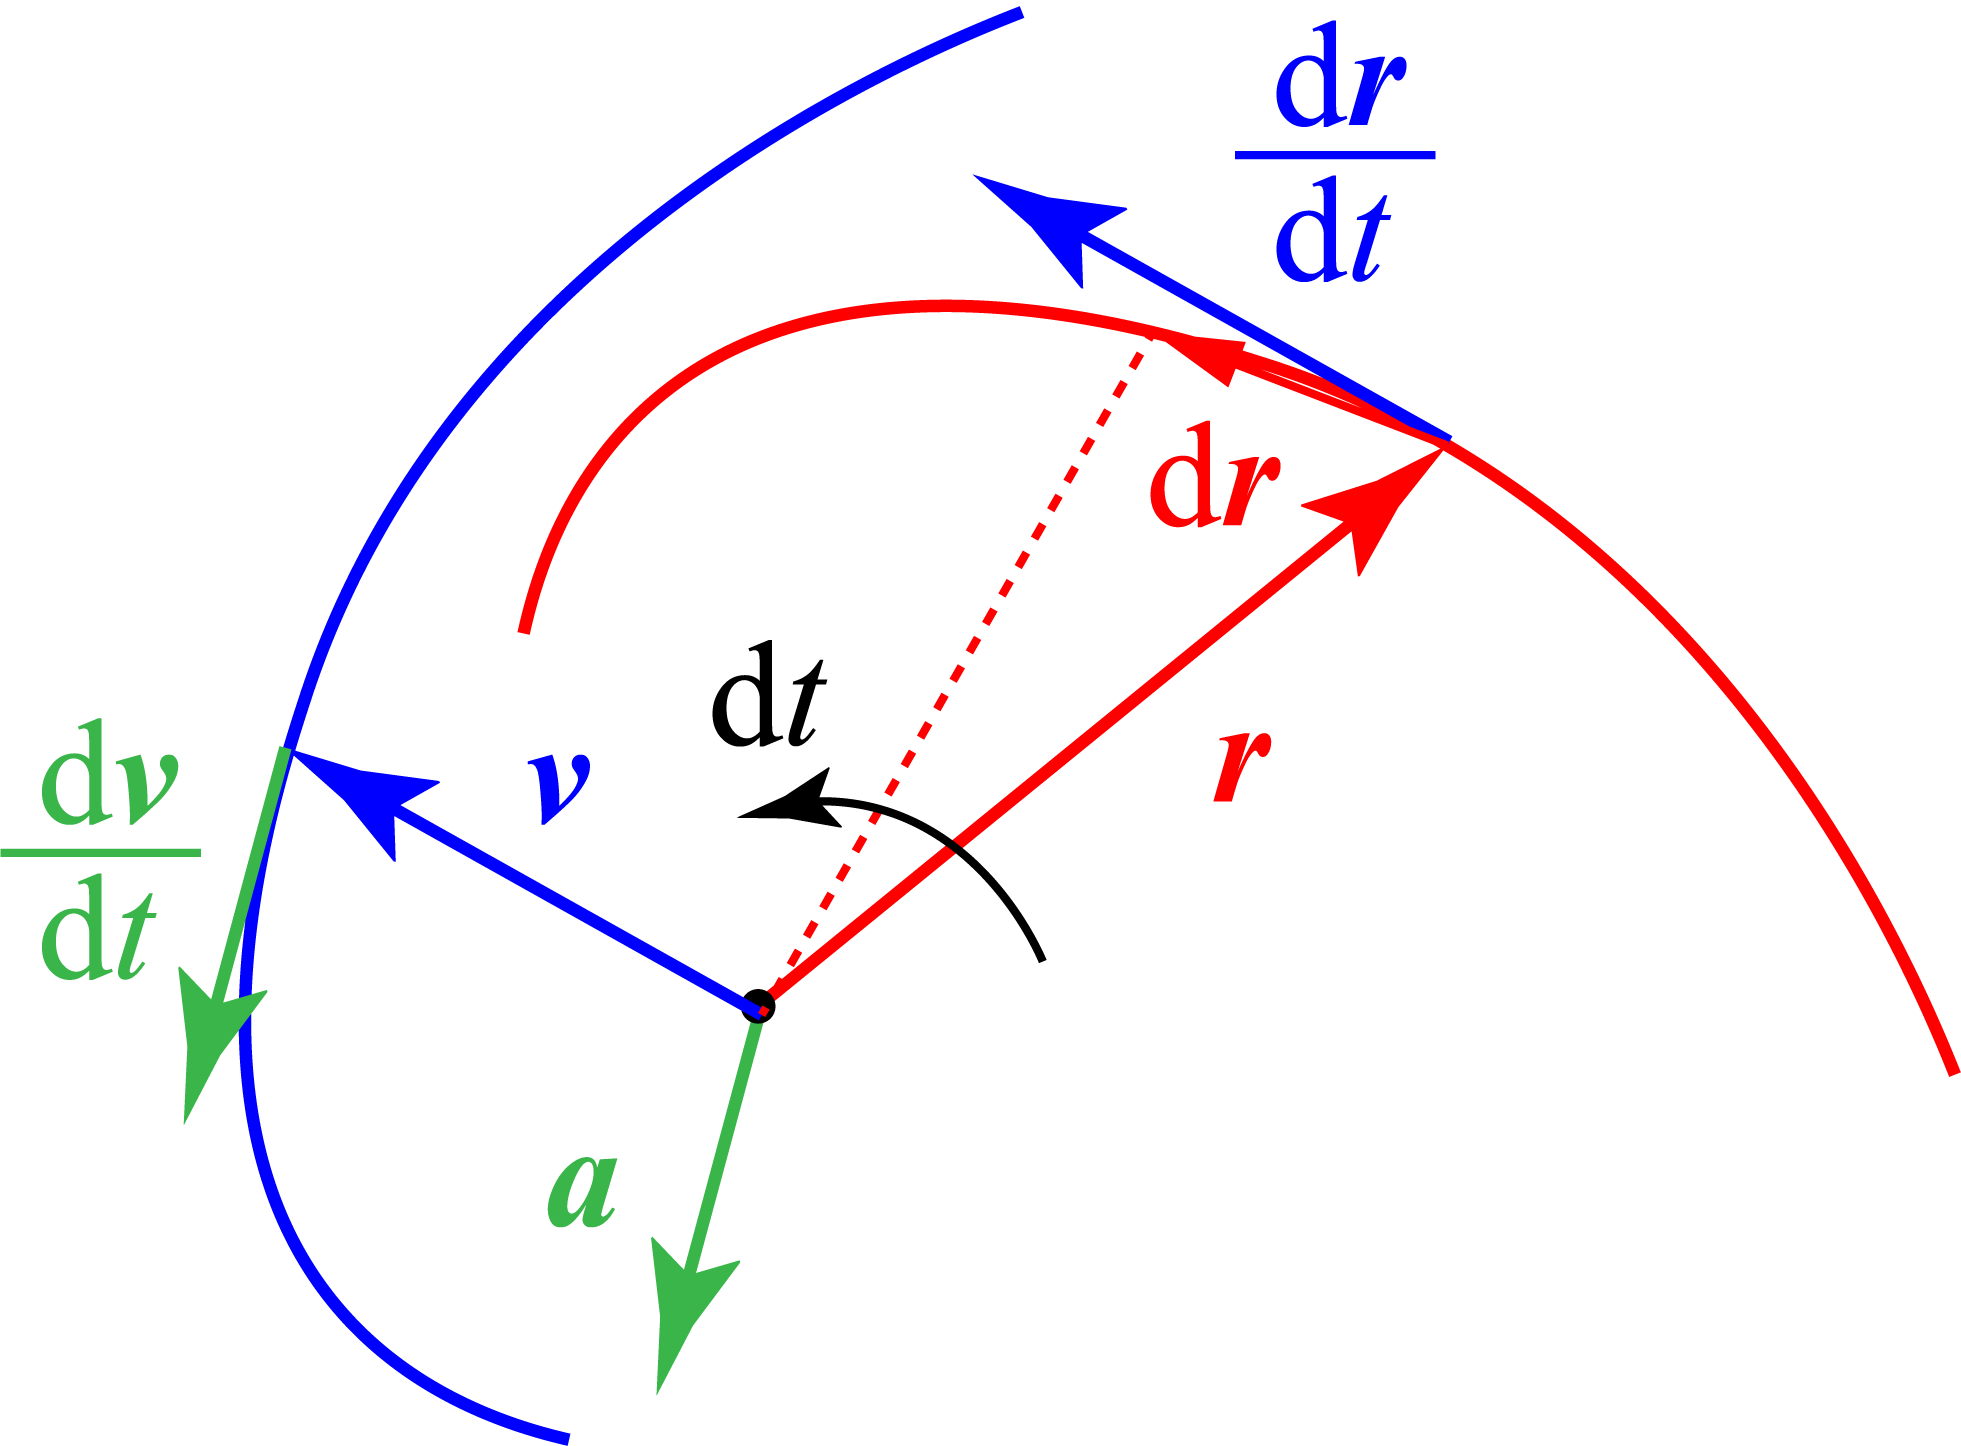
\includegraphics[width=7cm]{image/6-1-3.png}
\caption{质点的位置,\,速度与加速度}
\end{wrapfigure}
前者对应二维运动,\,后者对应三维运动.\,我们从中可以发现,\,函数是描述运动的数学工具,\,对矢量与函数的分析学知识便是运动学和物理学的基础.\,而运动学本身是可以看成是数学的一个分支的.\,对质点的位置矢量求导数便得到速度矢量,\,再求导数或是求二阶导数便是加速度矢量:
\[\bs{v}=\frac{\ud \bs{r}}{\ud t}=\lim_{\Delta t\to 0 }\frac{\bs{r}(t+\Delta t)-\bs{r}(t)}{\Delta t}\]
\[\bs{a}=\frac{\ud \bs{v}}{\ud t}=\lim_{\Delta t\to 0 }\frac{\bs{v}(t+\Delta t)-\bs{v}(t)}{\Delta t}\]
\[\bs{a}=\frac{\ud ^2\bs{r}}{\ud t^2}=\lim_{\Delta t\to 0 }\frac{[\bs{r}(t+\Delta t)-\bs{r}(t)]-[\bs{r}(t)-\bs{r}(t-\Delta t)]}{\Delta t^2}\]

正如上图\ref{6-1-3}所示,\,我们可以把每一个瞬时的速度矢量共起点画出来,\,并把端点连做曲线,\,此时背景的空间往往叫做\emph{速度空间}(velocity space),\,它的更普遍的对应是动量空间,\,这在近代物理的理论值具有重要地位.\,引入速度空间后质点的运动便可以等价地在速度空间中进行研究.\,比如在均匀重力场中的抛体运动在速度空间中就是简单的竖直向下的匀速直线运动.\,而平方反比力下的天体运动(开普勒问题)实际上在速度空间中可以证明将变为变速偏心圆周运动.\,这使得通过速度求加速度就好像通过位置求速度那样方便.\,具体求法接下来还得进一步展开.

加速度的导数偶尔也会进入物理研究的视野,\,它被叫做\emph{急动度}(jerk).\,即:
\[\bs{j}=\frac{\ud \bs{a}}{\ud t}=\frac{\ud ^3\bs{r}}{\ud t^3}\]

矢量函数概念就是实数到矢量的映射,\,但是具体能写出函数形式的例子在物理中却不是那么常见.\,比如抛体运动的运动对应的函数,\,即\emph{运动方程}(equation of motion)\footnote{指运动学运动方程,\,动力学运动方程就是反应运动的规律的,\,能够最终解出来运动学运动方程的微分方程.}为:
\[\bs{r}=\bs{r}_0+\bs{v}_0 t+\frac{1}{2}\bs{g}t^2\]

它是牛顿定律下以下微分方程结论的解:
\[\bs{a}=\frac{\ud ^2\bs{r}}{\ud t^2}=\bs{g}\]

但是在一般情况下,\,要表示出一个既有大小又有方向的矢量函数,\,我们得采用分解的思想,\,研究能够完全确定这个矢量值的参数.\,通常有以下做法:

\vspace{0.2cm}
{\bf 1.\,直角坐标系下的分解}

在一个欧几里得空间里的一个参考系中研究问题,\,很常见的一种做法是建立直角坐标系来表示一个点的位置.\,以更普遍的三维运动为例.\,既然物体的位置由坐标$(x,\,y,\,z)$来表示.\,我们就能认为表示运动的任务由三个标量函数$x(t),\,y(t),\,z(t)$来承担.\,其实这与上面介绍的用矢量来表示位置是非常一致的,\,因为实际上点的坐标通常也被理解为原点指向这个点的矢量在三个基矢的坐标:
\[\bs{r}=(x,\,y,\,z)=x\bs{i}+y\bs{j}+z\bs{k}\]

出于哈密顿(Hamilton)爵士关于把三维空间三个方向基矢视作四元数代数运算的旋转等效的奇妙观点,\,我们分别把$x,\,y,\,z$方向的基矢按照惯例记做$\bs{i},\,\bs{j},\,\bs{k}$.\,也常常因为它们是单位矢量(长度为1),\,而记做$\bs{e}_x,\,\bs{e}_y,\,\bs{e}_z$.\,这样便能把$\bs{r}$分解出$x$,\,$y$,\,$z$来.

分解以后,\,重新合成便能得到需要的物理量.\,这其中的意思是:\,比如我们为了求一个曲线运动速度或者加速度的$x$分量.\,也就是求下列表达式:
\[\bs{v}=v_x\bs{i}+v_y\bs{j}+v_x\bs{k}=\frac{\ud \bs{r}}{\ud t}\]
\[\bs{a}=a_x\bs{i}+a_y\bs{j}+a_x\bs{k}=\frac{\ud^2 \bs{r}}{\ud t^2}\]

中的分量$v_x,\,a_x$.\,其求法非常直接,\,便是:
\[v_x=\frac{\ud }{\ud t}x(t)\quad,\quad a_x=\frac{\ud^2 }{\ud t^2}x(t)\]

这相当于是说,\,求导数和向某固定方向投影是可以交换前后次序的:

\[\bs{i}\cdot \frac{\ud }{\ud t}\bs{r}=\frac{\ud }{\ud t}(\bs{i}\cdot \bs{r})\quad,\quad \bs{i}\cdot \frac{\ud }{\ud t}\bs{v}=\frac{\ud }{\ud t}(\bs{i}\cdot \bs{v})\]

这是当然的,\,因为矢量点乘的导数的法则也符合与标量乘积求导数类似的莱布尼茨法则,\,而常矢量$\bs{i}$不随着运动改变.\,所以导数只有对$\bs{r},\,\bs{v}$求导的项.

在数学上,\,曲线段也经常被描述为是与某实数上区间\emph{同胚}(homeomorphic)的几何图形,\,这其实就是说,\,存在自变量$t$,\,不失一般性地,\,我们让其取值范围为$(-\infty,\,+\infty)$.\,而存在一个从这个自变量到三维空间点$(x,\,y,\,z)$的光滑映射:
\[x=x(t)\quad ,\quad y=y(t)\quad ,\quad z=z(t)\]

\begin{wrapfigure}[10]{o}[-10pt]{7cm}\label{6-1-4}
\vspace{-0.4cm}
\centering
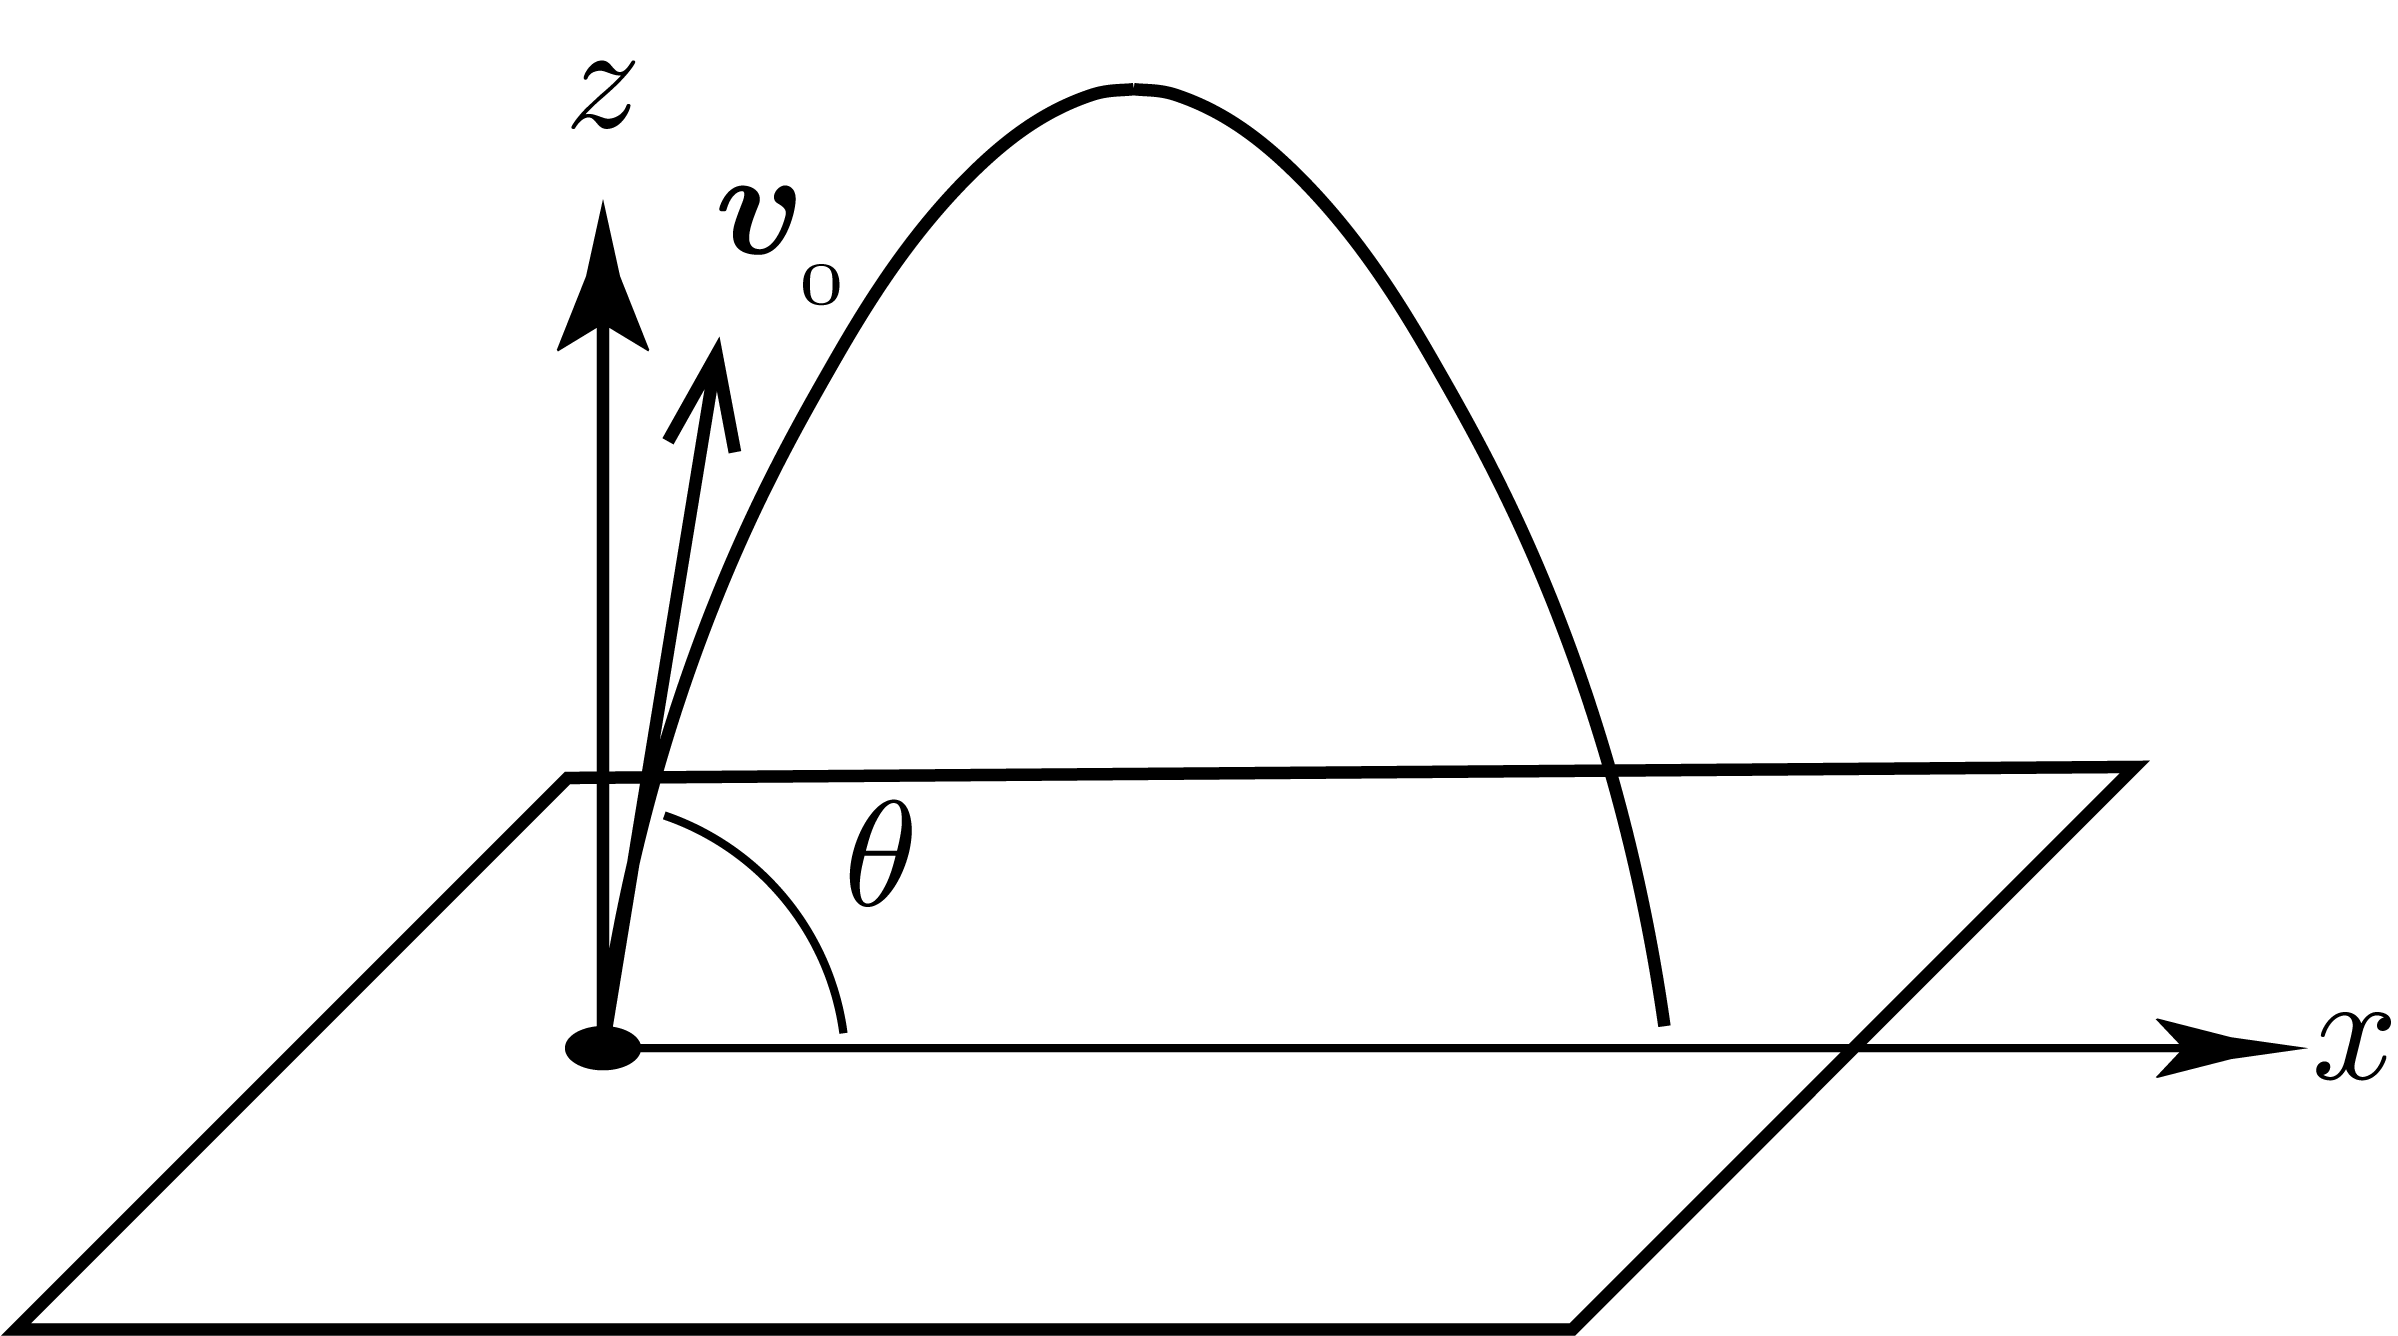
\includegraphics[width=7cm]{image/6-1-4.png}
\caption{抛体运动}
\end{wrapfigure}
在数学上看,\,这其实就是曲线方程:\,其参数方程的唯一给法.\,这样的式子就给出了几何学上的光滑曲线的定义.\,而不同于以往我们对曲线是$y=f(x)$的图像的刻板认识.\,但在这里,\,我们恰巧发现如果把参数$t$理解为时间的话,\,这恰好就对应到了一个粒子在三维空间中的运动,\,出于这样的原因,\,我们把反应了粒子位置随着时间变化的方程称为运动方程.\,它是\emph{轨迹方程}(function of trajactory)的一种特殊情况.\,对于轨迹方程,\,我们只需要通过符合方程的点$(x,\,y,\,z)$构成粒子所有运动中经过的位置构成的集合即可.\,例如,\,在地面$z=0$出发以仰角$\varphi$斜抛一个物体.\,那就以出发点为原点建立坐标系,\,竖直向上为$z$轴,\,抛的方向向前为$x$轴.\,那么运动方程为:
\[\left\{\begin{array}{l} x=v_0 t\cos\varphi\\ z=v_0 t\sin\varphi - \dfrac{1}{2}gt^2\end{array}\right.\]

但是轨迹方程不仅可以写成以上形式,\,还可以消去$t$得到:
\[z=x\tan\varphi -\frac{gx^2}{2v_0^2}(1+\tan^2\varphi)\]

\vspace{0.2cm}
{\bf 2.\,平面极坐标系下的分解}

如果质点做平面运动,\,那么我们问题得到了简化.\,此时往往有些情形下我们关心从原点的观察者出发看质点的运动时,\,质点离观察者的距离和质点相对观察者的方位.\,故引入\emph{极坐标系}(polar coordinate system)是自然而然的做法.\,其步骤为:\,确定观察者位置为\emph{极点}(pole),\,引出一条原点出发的射线为\emph{极轴}(polar axis);\,测量质点位置到极点距离$r$为\emph{矢径}(radius);\,从极点指向质点位置形成矢量矢径$\bs{r}$,\,测量极轴绕极点沿指定的正方向旋转到与矢径重合时旋转的角度$\theta$为\emph{极角}(polar angle).\,描述质点的位置时,\,$(r,\,\theta)$即构成极坐标.

仍然,\,极坐标可以用来表示质点的唯一位置:\,只需要给出$(r,\,\theta)$就可以确定位置.\,所以只要知道函数$r(t),\,\theta(t)$就能够确定其运动,\,这便是极坐标下的运动方程.\,同理如果消去$t$就能得到另一类轨迹方程.\,只要物体运动轨迹不经过极点,\,我们总是取$r(t),\,\theta(t)$为光滑的函数.\,$\theta$的取值为$(-\infty,\,+\infty)$以保证运动的连续性.\,不过$\theta$相差$2k\pi,\,k\in\mathbb{Z}$的所有坐标表示运动过程中的同一位置.

例如,\,在之前的抛体运动中,\,如果取$z$轴为极轴,\,那么其极坐标下的运动方程为:
\[\left\{\begin{array}{l} r^2=(\bs{v}_0 t+\dfrac{1}{2}\bs{g}t^2)^2=\dfrac{1}{4}g^2t^4  -gv_0t^3\sin\varphi + v_0^2t^2\\[3pt] \tan\theta=\dfrac{2v_0 \cos\varphi}{2v_0 \sin\varphi-gt}\end{array}\right.\]

这会有利于我们分析一些问题.\,例如如果关心以何种倾角抛出一个物体,\,物体离我们的距离会越来越远?\,就只需要让$r$为关于$t$的增函数,\,除了对$r$求导的做法,\,一种更加明智的做法可能是注意到关系式:
\[\frac{\ud r}{\ud t}>0  \quad\Leftrightarrow\quad	\frac{\ud}{\ud t}(\frac{1}{2}r^2)>0\]
\begin{align*} 
\Leftrightarrow \frac{\ud}{\ud t}(\frac{1}{2}r^2)	&=\frac{\ud}{\ud t}(\frac{1}{2}{\bs{r}\cdot\bs{r}})=\bs{r}\cdot\bs{v}\\
																			&=(\bs{v}_0 t+\dfrac{1}{2}\bs{g}t^2)\cdot(\bs{v}_0 +\bs{g}t)>0\\
\end{align*}

\[\Leftrightarrow (\bs{v}_0 +\dfrac{1}{2}\bs{g}t)\cdot(\bs{v}_0 +\bs{g}t)=\dfrac{1}{2}g^2t^2  -\dfrac{3}{2}gv_0t\sin\varphi + v_0^2>0\]

这就化为求关于$t$的二次函数恒大于零的系数条件问题,\,结论是初等的:\,判别式小于零:
\[\left(\dfrac{3}{2}gv_0\sin\varphi\right)^2-4\left(\dfrac{1}{2}g^2 \right)(v_0^2)<0\quad \Rightarrow\quad \sin\varphi<\frac{2\sqrt{2}}{3}\]

\begin{wrapfigure}[12]{o}[-10pt]{6cm}\label{6-1-5}
\vspace{-0.4cm}
\centering
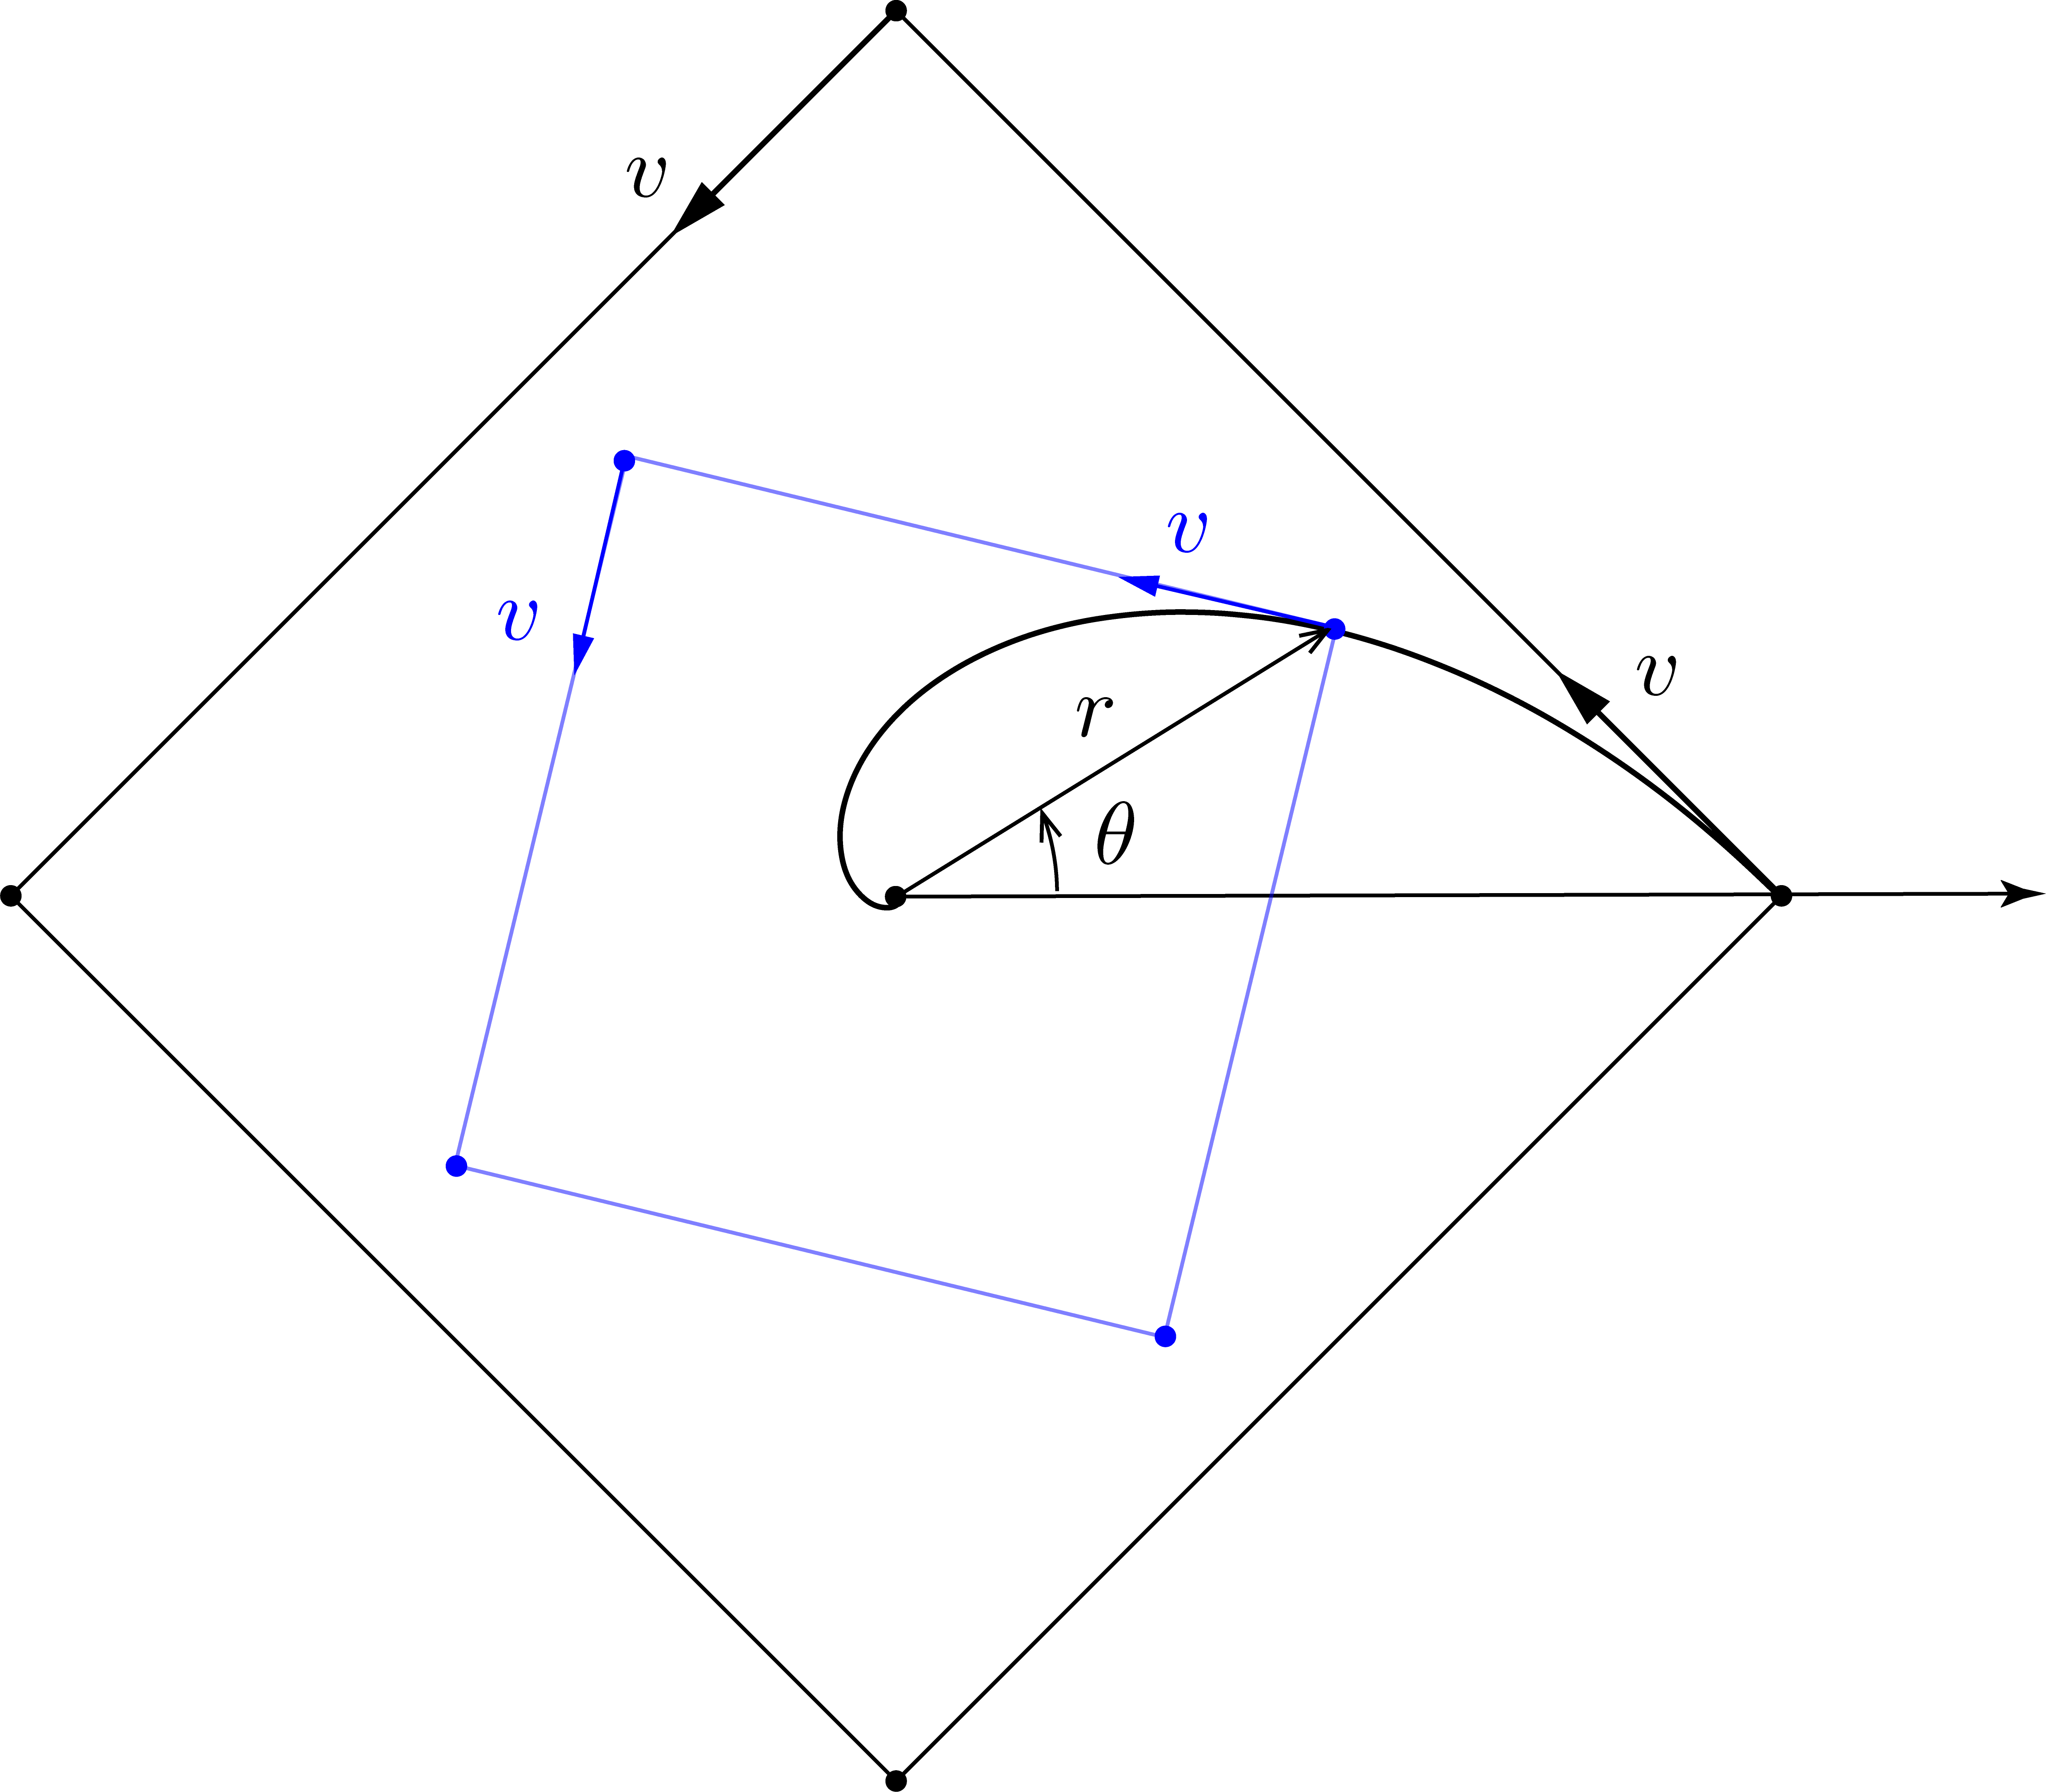
\includegraphics[width=6cm]{image/6-1-5.png}
\caption{首尾相追}
\end{wrapfigure}
采用极坐标系描述抛体运动也许是费力而不讨好的.\,但是描述其他一些运动又比直角坐标系存在天然的优势.\,比如一类经典追击问题的表述如下:\,四个平面运动的质点初始组成正方形.\,这个环形的结构中每一个质点都向着前一个质点运动发生追击.\,其中运动速度矢量具有变化的方向,\,即向着前方质点.\,但具有不变的速率$v$.\,确定物体的运动方程和轨迹.

对于这个问题,\,预先的关于物体在时间为$t$时的位置信息是几乎完全空缺的,\,但对于速度矢量我们知道一个信息:\,其大小为$v$.\,如果考虑直角坐标系,\,这个条件表示为:
\[|\bs{v}|=\sqrt{\dot{x}^2+\dot{y}^2}=v\]

但是对于位置和速度,\,我们还知道一个信息,\,就是它们夹钝角而且为$3\pi/4$.\,用直角坐标系的公式仔细化简的话也可以得到:
\[\tan \phi_{\bs{r}\curvearrowright \bs{v}}=-1\quad \Rightarrow \quad \frac{\bs{r}\cdot\bs{v}}{|\bs{r}\times \bs{v}|}=\frac{x\dot{x}+y\dot{y}}{x\dot{y}-y\dot{x}}=-1\]

\begin{wrapfigure}[12]{o}[-10pt]{6cm}\label{6-1-6}
\vspace{-0.4cm}
\centering
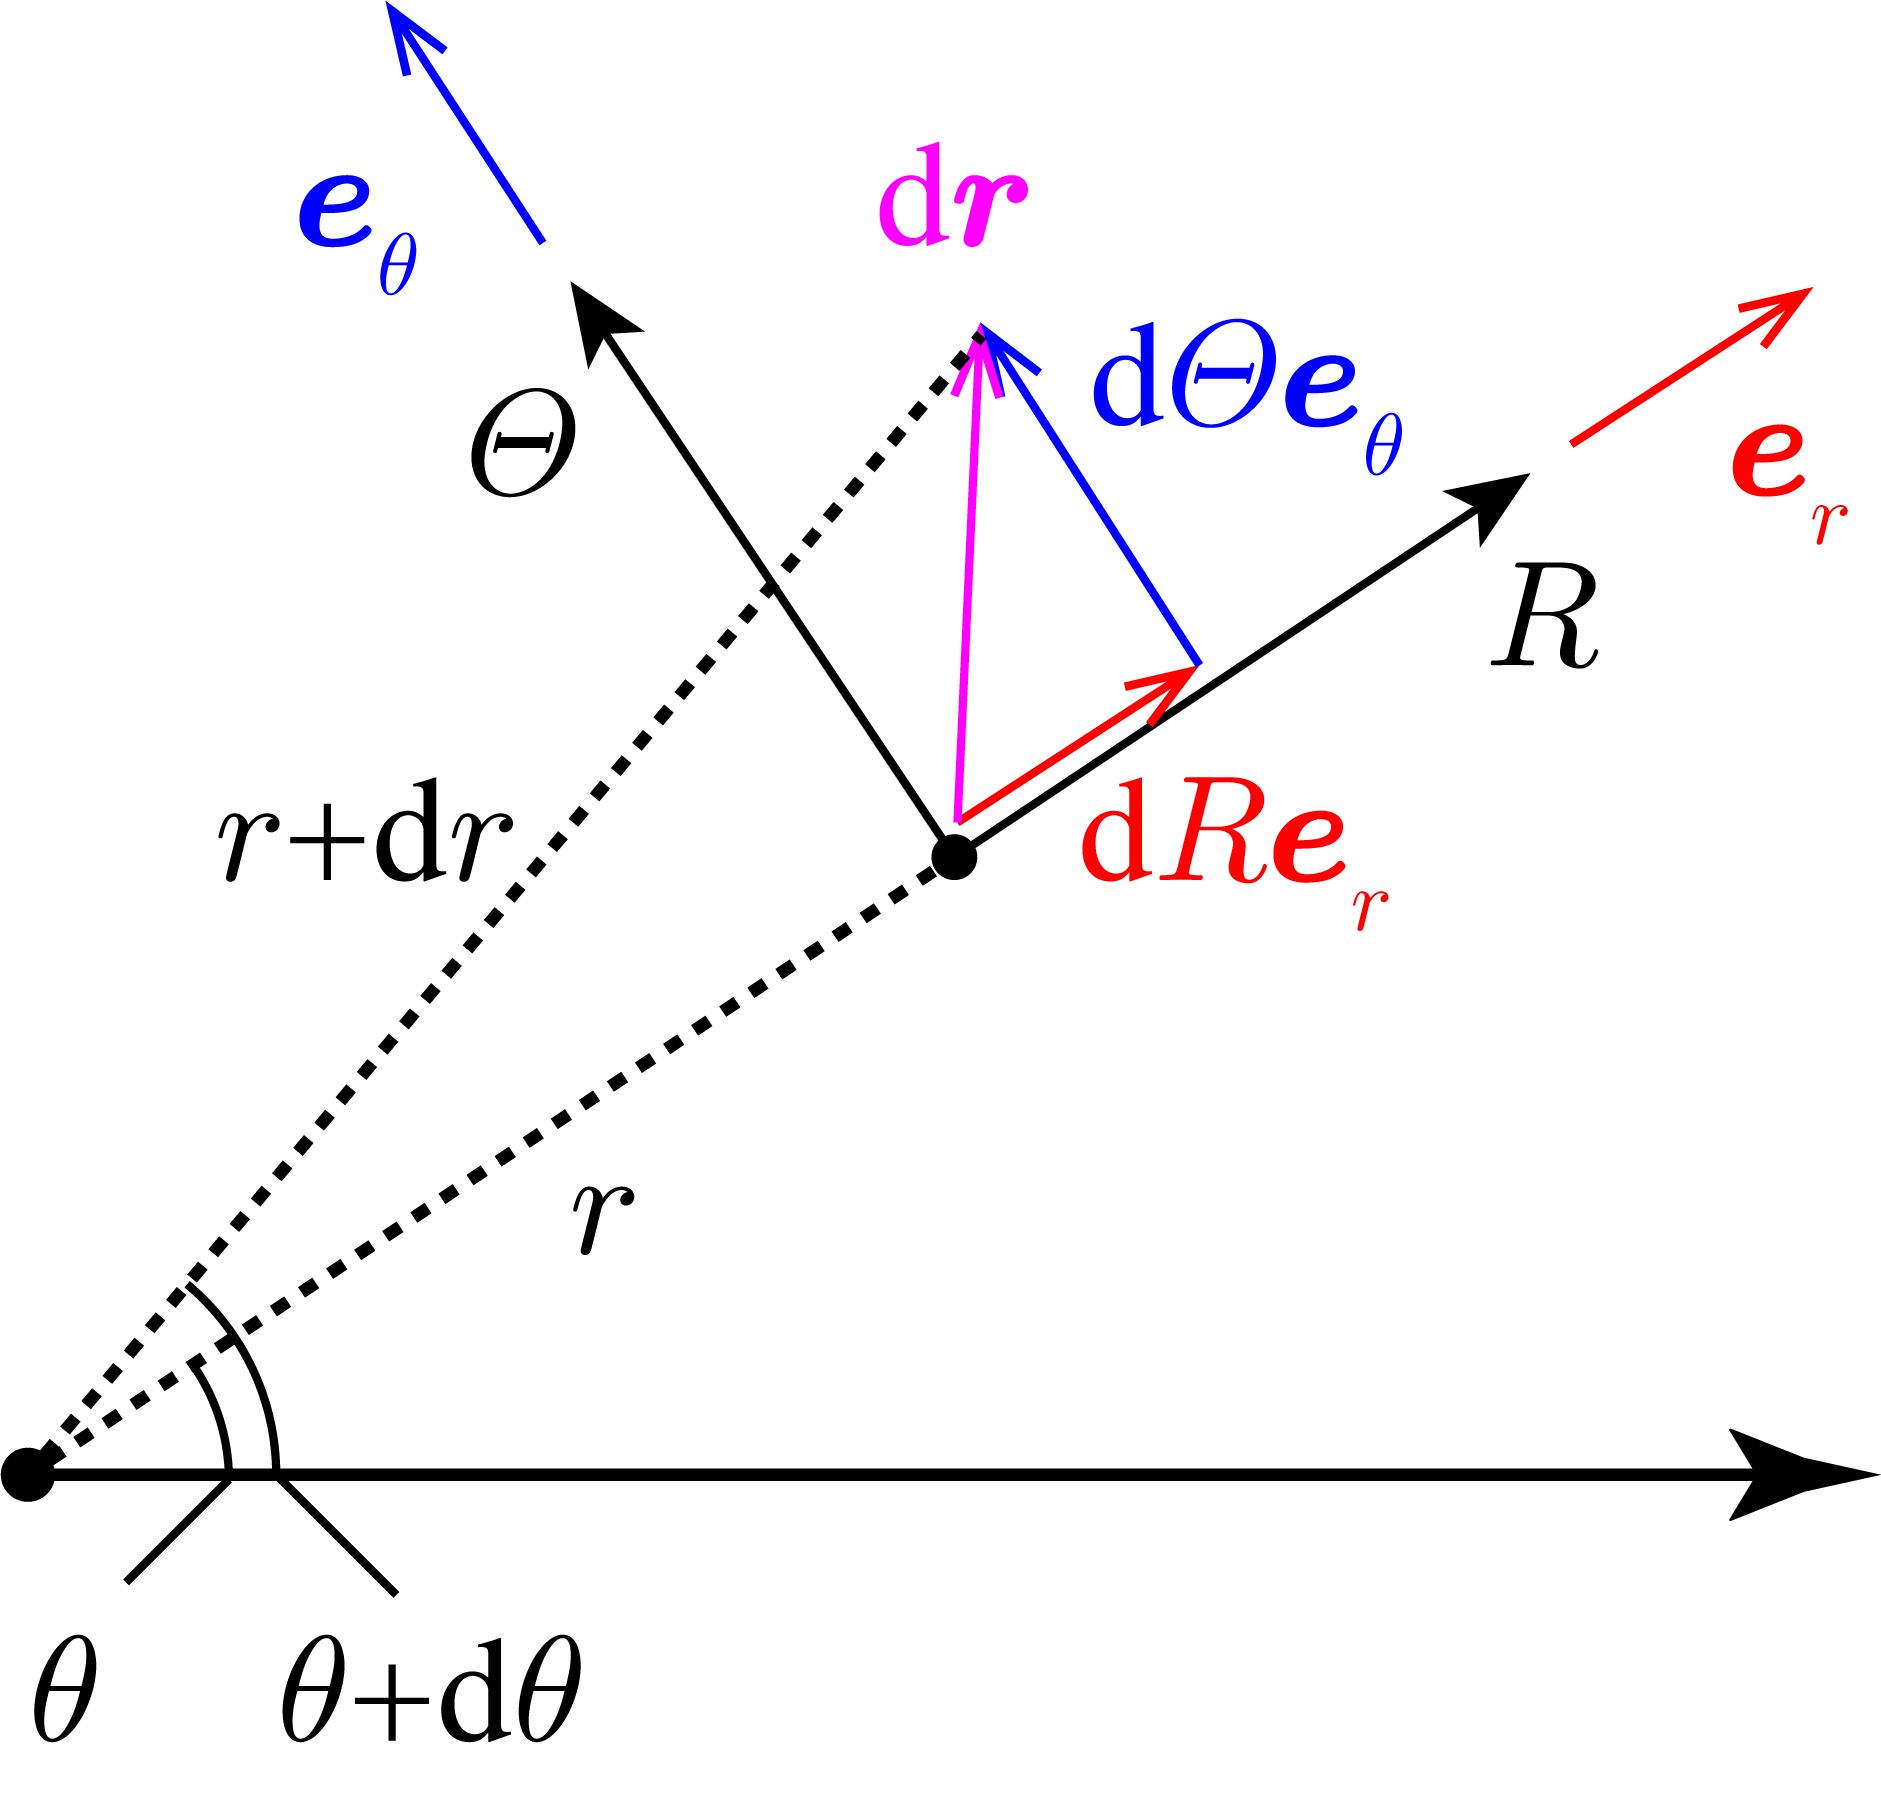
\includegraphics[width=6cm]{image/6-1-6.png}
\caption{极坐标系的活动框架}
\end{wrapfigure}
但这就较难求解\footnote{有兴趣的读者可以挑战一下.}.\,那么如果采用极坐标系会为我们带来何种新的思路呢?

那就是\emph{活动标架}(moving frame)的引入.\,无论粒子在何处,\,粒子的$\bs{r}$一定是作为了$r$和$\theta$的函数的.\,那么可以在粒子所在的点沿两个方向建立局域的$R-\varTheta$直角坐标系.\,这两个方向怎么确定呢?\,其实就是基矢的方向:
\[\bs{e}_r:=\frac{\partial\bs{r}}{\partial r}\left/\middle|\frac{\partial\bs{r}}{\partial r}\right|=\frac{\partial\bs{r}}{\partial r}\quad,\quad \bs{e}_\theta:=\frac{\partial\bs{r}}{\partial \theta}\left/\middle|\frac{\partial\bs{r}}{\partial \theta}\right|=\frac{1}{r}\frac{\partial\bs{r}}{\partial \theta}\]

上式中后一个偏导数的模为$r$是显然的.\,只需要考虑到圆的弧长和半径的关系即可.

局域的标架给我们什么方便?\,我们由偏导数和全微分的法则可以描述局域物体的微小位移.\,本质上,\,这相当于$\ud r$和$\ud \theta$导致的位矢$\bs{r}$改变$\ud \bs{r}$:
\[\ud \bs{r}_{(\ud r,\,\ud \theta)}=\ud \bs{r}_{(\ud r,\,0)}+\ud \bs{r}_{(0,\,\ud \theta)}=\ud R\bs{e}_r+\ud \varTheta\bs{e}_\theta\]
\[\ud \bs{r}_{(\ud r,\,\ud \theta)}=\frac{\partial \bs{r}}{\partial r}\ud r+\frac{\partial \bs{r}}{\partial \theta}\ud \theta=\ud r\bs{e}_r+r\ud \theta \bs{e}_\theta\]
\[\Rightarrow \quad \ud R=\ud r\;,\;\ud \varTheta=r\ud \theta\]

可见在曲线坐标情形下坐标的改变量$\ud r,\,\ud \theta$与在对应质点位移方向走过的弧长$\ud R,\,\ud \varTheta$的值一般是不一样的.\,它们之前的比值(弧长/坐标变化)称作\emph{拉梅系数}(Lam\'e coefficient).

\vspace{0.5cm}
既然叫做活动标架法,\,那么显然随着粒子的运动,\,两个基矢$\bs{e}_r,\,\bs{e}_\theta$的方向也在不断改变中.\,我们用极坐标,\,就是把一个物理量$\bs{A}$分解到粒子运动的瞬时局域坐标系中:
\[\bs{A}=A_r\bs{e}_r+A_\theta\bs{e}_\theta\]

那么在粒子发生运动后,\,以上矢量的改变应当由四部分组合而成:
\[\ud \bs{A}=\ud'\bs{A}+\tilde{\ud}\bs{A} \]
\[\ud' \bs{A}:=\ud A_r\bs{e}_r+\ud A_\theta\bs{e}_\theta\]
\[\tilde{\ud}\bs{A}:= A_r\ud\bs{e}_r+ A_\theta\ud\bs{e}_\theta\]

其中$\ud'$表示相对变化,\,类似于选取跟随旋转的活动标架而旋转的参考系后,\,矢量的变化量,\,故基矢自己的变化是被无视了的.\,而原来的$\ud$才表示绝对的变化.\,而$\tilde{\ud}$所带来的变化称作牵连变化或随体变化.\,它是即使前面的相对变化为零也会带来的,\,由于标架的``拉拽''导致的旋转带来的改变.\,事实上很容易证明其中的:
\[\ud \bs{e}_r=\ud \bs{\theta}\times \bs{e}_r=+\ud \theta \bs{e}_\theta\]
\[\ud \bs{e}_\theta=\ud \bs{\theta}\times \bs{e}_\theta=-\ud \theta \bs{e}_r\]

其中$\ud \bs{\theta}$是方向垂直于纸面向外的,\,大小即极坐标下物体坐标之角坐标的增量$\ud \theta$.

这就足以给出:
\[(\ud \bs{A})_r=\ud A_r-A_\theta \ud \theta\]
\[(\ud \bs{A})_\theta=\ud A_\theta+A_r \ud \theta\]
\newpage
两边再同时除以时间,\,我们得到粒子运动过程中一个矢量导数的两个分量与这矢量两个分量的导数之间的关系:
\[(\dot{\bs{A}})_r=\dot{A_r}-\dot{\theta}A_\theta\]
\[(\dot{\bs{A}})_\theta=\dot{A_\theta}+\dot{\theta}A_r\]

导数的分量不等于分量的导数,\,这也是坐标系的弯曲所带来的.\,数学上,\,这意味算符$\partial_t$与算符$\bs{e}\cdot$的\emph{不对易性}(non-commutative):
\[\bs{e}\cdot(\partial_t \bs{A})\neq \partial_t(\bs{e}\cdot \bs{A})\]

通过这个原理,\,我们可以推理得到:
\[\bs{r}=r\bs{e}_r+0\bs{e}_\theta\quad \Rightarrow\quad r_r=r\,,\,r_\theta=0\]
\[\bs{v}=\dot{\bs{r}}\quad \Rightarrow\quad  v_r=\dot{r_r}-\dot{\theta}r_\theta=\dot{r}\,,\,v_\theta=\dot{r_\theta}+\dot{\theta}r_r=\dot{\theta}r\]
\[\bs{a}=\dot{\bs{v}}\quad \Rightarrow\quad  a_r=\dot{v_r}-\dot{\theta}v_\theta=\ddot{r}-\dot{\theta}^2r\,,\,a_\theta=\dot{v_\theta}+\dot{\theta}v_r=\ddot{\theta}r+2\dot{\theta}\dot{r}\]

这个操作甚至可以继续下去,\,计算急动度等:
\[\bs{j}=\dot{\bs{a}}\quad \Rightarrow \quad j_r=\dot{a_r}-\dot{\theta}a_\theta=\dddot{r}-3\dot{\theta}\ddot{\theta}r-3\dot{\theta}^2\dot{r}\,,\,j_\theta=\dot{a_\theta}+\dot{\theta}a_r=\dddot{\theta}r+3\ddot{\theta}\dot{r}+3\dot{\theta}\ddot{r}-\dot{\theta}^3r\]
\[\cdots\]

极坐标下速度,\,加速度的公式是非常常用的,\,它们是:
\[\bs{v}=(\dot{r}\,,\,\dot{\theta}r)\quad\bs{a}=(\ddot{r}-\dot{\theta}^2r\,,\,\ddot{\theta}r+2\dot{\theta}\dot{r})\]

故,\,在之前的首尾相追问题\ref{6-1-5}中以正方形中心为原点,\,以初始位置为极轴方向建立极坐标系.\,那么两个条件:\,速度大小恒定为$v$和位矢速度夹角恒定$3\pi/4$表述为:
\[v_r^2+v_\theta^2=v^2\quad ,\quad \frac{v_\theta}{v_r}=-1\]

相当容易解出来两个分速度的值,\,再结合之前的速度公式:
\[\dot{r}=-\frac{\sqrt{2}}{2}v\quad ,\quad \dot{\theta}r=\frac{\sqrt{2}}{2}v\]

这样,\,便可以轻松解出运动方程来,\,结合初始条件,\,不妨设初始矢径为$r_0$,\,幅角为$0$:
\[\dot{r}=-\frac{v}{\sqrt{2}}\quad \Rightarrow \quad r=r_0-\frac{vt}{\sqrt{2}}\]
\[\dot{\theta}=\frac{v}{\sqrt{2}r_0-vt}\quad \Rightarrow \quad  \theta =-\ln\left(1-\frac{vt}{\sqrt{2}r_0}\right)\]

轨迹方程通过上述方程消参即可.\,但也可以通过之前的微分方程相除得到新微分方程求解,\,曲线为\emph{对数螺线}(logarithmic spiral):
\[\frac{\ud r}{\ud \theta}=-r\quad \Rightarrow \quad r=r_0\ue^{-\theta}\]

平面的极坐标系在三维空间的推广为\emph{柱坐标系}(cylindrical coordinate system)和\emph{球坐标系}(spherical coordinate system).\,类似公式的核心也与平面极坐标相差无几,\,都在于活动标架的基矢微分.\,请读者自行推导.

\vspace{0.2cm}
{\bf 3.\,自然坐标系下的分解}

设想仍然采用活动标架法的思路,\,但是,\,标架的方向不再由粒子的位置相对事先建立的背景的坐标系的关系而决定.\,而是紧密地由粒子运动的性质:\,瞬时的速度方向,\,轨迹曲线的弯曲方向等决定.\,那么我们就得到了特殊的标架:\,\emph{自然坐标系}(natural coordinates).

自然坐标系的建立是派生于粒子运动的轨迹的那条曲线的性质的.\,借助牛顿等人创立的微积分与笛卡尔等人创立的解析几何的帮助,\,对于光滑曲线曲面的性质的研究构成了\emph{古典微分几何}(classical differential geometry)的主要课题.\,

我们考虑三维空间问题.\,对于一条空间曲线.\,它总是一些点的集合,\,而如果规定某个起始点以后,\,每一个点都会有一个$s$坐标,\,它就是从起始点到这个点的弧长.\,而其实我们可以把$s$视作一个自变量,\,因为$s$改变而改变的是不同点的位置$\bs{r}$.\,也就是说$\bs{r}(s)$作为了$s$的函数.\,那么这个曲线在某一点处的切矢量就可以被自然地定义为:
\[\bs{\tau}=\frac{\ud \bs{r}}{\ud s}\]

\begin{wrapfigure}[14]{o}[-10pt]{6cm}\label{6-1-7}
\vspace{-0.2cm}
\centering
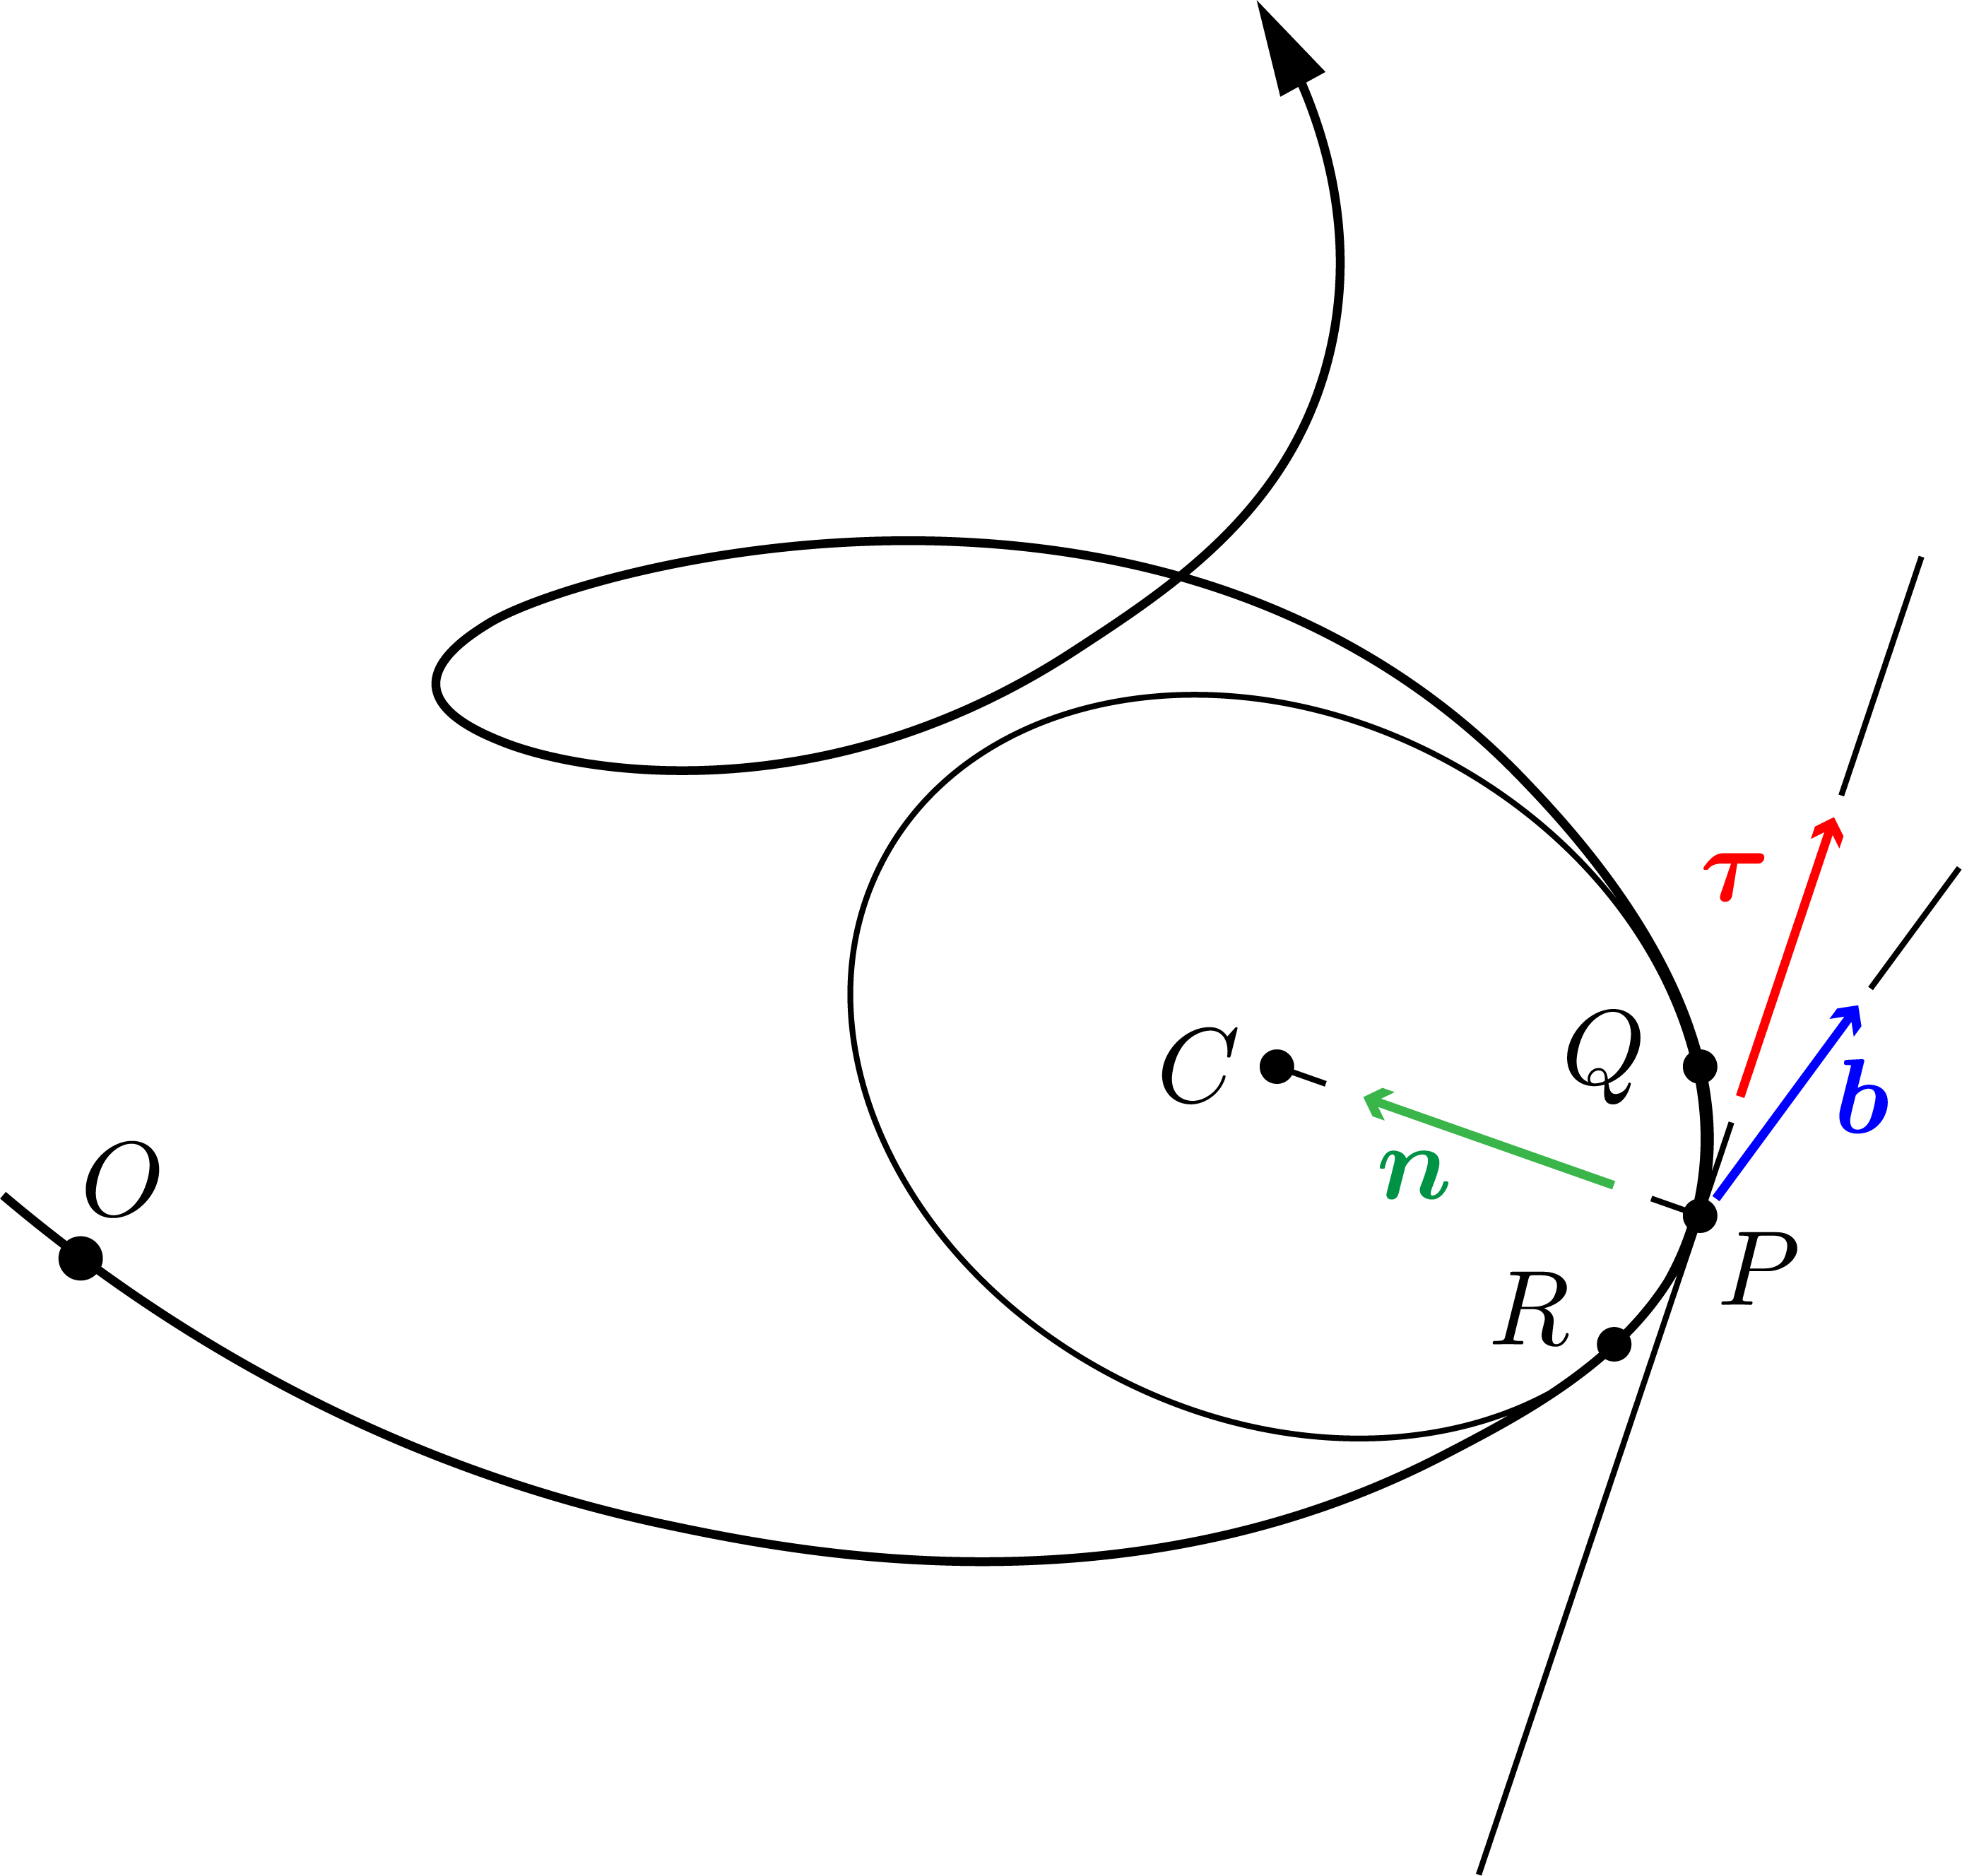
\includegraphics[width=6cm]{image/6-1-7.png}
\caption{Frenet框架}
\end{wrapfigure}
以上矢量模自然为$1$.\,因为分子$\ud \bs{r}$的长度就是分母的$\ud s$.\,方向则是在曲线的\emph{切线}(tangent line)方向.\,切线是这样一种线:\,曲线上有一点$P$.\,如果在$P$两侧任取一个点$Q$并连接$PQ$,\,使$Q$无限接近$P$即$\ud s \to 0$,\,那么$PQ$所在的直线的极限就是$P$点的切线.\,这又引申出第二个概念:\,如果在$P$所有各取一个点$Q,\,R$.\,那么$PQR$三点确定的圆也将随着$Q,\,R$同时无限接近于$P$而具有极限.\,这个圆叫做\emph{密切圆}或\emph{曲率圆}(osculating circle).\,其所在的平面叫做\emph{密切平面}(osculating plane).\,而圆心$C$为\emph{曲率中心}(center of curvature),\,最后,\,实际上$P$到$C$的方向就是\emph{法}(normal)方向,\,该方向的单位矢量叫做法矢量$\bs{n}$.\,而副法矢量$\bs{\tau}\times\bs{n}=\bs{\beta}$所决定的方向为\emph{副法}(binormal)方向.\,这样三个矢量便构成\emph{弗雷内框架}(Frenet frame)或称TNB框架.

事实上,\,如果计算曲线在过程中的转向,\,它可以用三个矢量方向的变化来表示.\,如果计算三个矢量对$\ud s$的变化率,\,一定能写作:
\[\begin{array}{rlll}
\frac{\ud \bs{\tau}}{\ud s}=		&	+0\bs{\tau} 	&	+k\bs{n} 		& +\varepsilon\bs{\beta}\\
\frac{\ud \bs{n}}{\ud s}=		&	-k\bs{\tau} 	&	+0\bs{n} 		& +\gamma\bs{\beta}\\
\frac{\ud \bs{\beta}}{\ud s}=		&	-\varepsilon\bs{\tau} 	&	-\gamma\bs{n} 		& +0\bs{\beta}
\end{array}\]

这是因为框架一定要具有正交归一的一套基矢量,\,而且这个性质在曲线上任何一点都要成立,\,指的是以下六个式子:
\[\bs{\tau}\cdot\bs{\tau}=1\quad,\quad\bs{n}\cdot\bs{n}=1\quad,\quad \bs{\beta}\cdot\bs{\beta}=1\]
\[\bs{\tau}\cdot\bs{n}=0\quad,\quad\bs{n}\cdot\bs{\beta}=0\quad,\quad \bs{\beta}\cdot\bs{\tau}=0\]

对六个式子分别求导数就看出来了,\,\emph{一个单位矢量自己的导数必然垂直于自身},\,从而三个基矢导数在自己上的投影都必须为零.\,而两个不同基矢的导数互相在对方方向的投影则会正负相消,\,这样才能保证两个矢量始终正交.\,就能理解之前的$9$个系数为什么要写成这个形式.

最后我们指出,\,系数$\varepsilon$应当是$0$.\,这是因为作为法线方向的定义本身,\,它就应当在$\bs{\tau}$的变化量$\ud\bs{\tau}$所在的方向上.\,从而第一个式子不会具有$\bs{\beta}$方向的分量.\,综上所述,\,我们得到了:

\[\begin{array}{rlll}
\frac{\ud \bs{\tau}}{\ud s}=		&	 	&	+k\bs{n} 		& \\
\frac{\ud \bs{n}}{\ud s}=		&	-k\bs{\tau} 	&	 		& +\gamma\bs{\beta}\\
\frac{\ud \bs{\beta}}{\ud s}=		&	 	&	-\gamma\bs{n} 		& 
\end{array}\]

这就是\emph{弗雷内公式}(Frenet formulae).\,其中$k$称作曲线的\emph{曲率}(curvature).\,它的意义是衡量了曲线方向转动的快慢,\,事实上由于曲线切线的无穷小转动角度其实在竖直上恰好会等于无穷小矢量$\ud\bs{\tau}$的长度,\,从而有:
\[k=\abs{\frac{\ud\bs{\tau}}{\ud s}}=\frac{\ud\theta}{\ud s}\]

即,\,曲率为:\,质点沿曲线走单位长度所转过的角度.\,曲率半径实际上是曲率的倒数.\,它是曲率圆的半径$\rho=1/k$.

而$\gamma$则被称作\emph{挠率}(torsion).\,我们通过弗雷内公式的第三式可以发现,\,挠率反映了副法矢量,\,或者说被复法矢量作为法平面的密切平面,\,绕曲线此时的切线的旋转快慢.\,它使得粒子瞬时运动的那个平面在改变着.\,下面我们会发现,\,实际上挠率对运动学中直到加速度的表达式都是没有任何贡献的.

如何用自然法描述粒子的运动?\,事实上这就相当于把粒子运动的路程$s$和三个矢量$\bs{\tau},\,\bs{n},\,\bs{\beta}$都表示为时间的函数:
\[s(t),\,\bs{\tau}(t),\,\bs{n}(t),\,\bs{\beta}(t)\]

但事实上,\,曲线本身轨迹必须先存在才能让我们事先确定好框架,\,而这样一个曲线其实本身由$\bs{r}(s)$给出,\,而且满足:
\[\frac{\ud \bs{r}}{\ud s}=\bs{\tau}\quad,\quad \frac{\ud^2 \bs{r}}{\ud s^2}=k\bs{n}\quad,\quad \frac{\ud^3 \bs{r}}{\ud s^3}=-k^2\bs{\tau}+\frac{\ud k}{\ud s}\bs{n}+k\gamma\bs{\beta}\]

然后我们唯一要做的就是给出$s(t)$函数,\,这一定可以帮助我们确定运动的各个量.

事实上,\,由于泰勒展开公式,\,近似到三阶:
\[\Delta \bs{r}\simeq\frac{\ud \bs{r}}{\ud s}\ud s+\frac{1}{2}\frac{\ud^2 \bs{r}}{\ud s^2}\ud s^2+\frac{1}{6}\frac{\ud^3 \bs{r}}{\ud s^3}\ud s^3=(k\ud s-\frac{k^2}{6}\ud s^3)\bs{\tau}+(\frac{k}{2}\ud s^2+\frac{1}{6}\frac{\ud k}{\ud s}\ud s^3)\bs{n}+\frac{k\gamma}{6}\ud s^3\bs{\beta}\]

如果只保留领头项,\,忽略高阶小量.\,我们就得到,\,在粒子运动的局域坐标系中,\,位移$\ud s$长度到达的点三个坐标$T,\,N,\,B$分别近似为:
\[T=\ud s \quad,\quad N=\frac{k}{2}\ud s^2 \quad,\quad B=\frac{k\gamma}{6}\ud s^3\]

仍然考虑之前的三阶近似下的严格$\Delta \bs{r}$与$\ud{s}$的关系,\,这一次代入$s(t)$的三阶套了展开:
\[\ud s\simeq \dot{s}\ud t+\frac{\ddot{s}}{2}\ud t^2+\frac{\dddot{s}}{6}\ud t^3\]

我们整理$\ud t$的各阶项,\,最终得到:
\[\Delta \bs{r}\simeq \bs{v}\ud t+\frac{1}{2}\bs{a}\ud t^2+\frac{1}{6}\bs{j}\ud t^3\]

其中速度与加速度的公式为:
\[\bs{v}=\dot{s}\bs{\tau}\]
\[\bs{a}=\ddot{s}\bs{\tau}+k\dot{s}^2\bs{n}\]

速度方向必然沿切向,\,大小上就等于$\dot{s}$,\,即单位时间走过的弧长.\,而加速度则有两个分量.\,一是由于速率在增减导致的切向加速度,\,大小等于$a_\tau=\ddot{s}$;\,第二项则是由于曲线的弯曲导致的法向加速度.\,它的值为$a_n=\dot{s}^2/\rho$.\,

如果要计算急动度等,\,可以从之前的泰勒展示中获得,\,其实还可以直接对加速度求导数,\,此时表达式会突然产生很多项:
\[\bs{j}=(\dddot{s}-k^2\dot{s}^3)\bs{\tau}+(3k\dot{s}\ddot{s}+\dot{k}\dot{s}^3)\bs{n}+k\gamma\dot{s}^3\bs{\beta}\]

利用自然坐标下的分解方式,\,如果已经直到特定曲线的曲率,\,就可以根据质点在曲线上的运动方式来计算运动的加速度.\,但是反过来利用运动学公式来确定曲线的曲率半径也不失为一种极其简单的做法.\,我们注意到,\,利用加速度在垂直于速度方向的那个分量即为$v^2/\rho$的结论,\,可以得到:
\[\rho=\frac{\bs{v}^3}{\abs{\bs{a}\times\bs{v}}}\]

例如,\,如果已知二维空间中的曲线方程$y=f(x)$.\,那么如果命一质点在曲线上运动且满足$x=t,\,y=f(t)$,\,那么速度为$\bs{v}=(1,\,f')$,\,加速度为$\bs{a}=(0,f'')$.\,利用上式可得:
\[\rho=\frac{(1+f'^2)^\frac{3}{2}}{\abs{f''}}\]

再例如.\,之前的首尾相追问题中,\,曲线对数螺线写作:
\[r=a\ue^{k\theta}\]

如何计算曲率半径?\,我们让粒子在曲线上绕极点做匀速旋转,\,也就是:
\[\theta=\omega t\quad,\quad r=a\ue^{k\omega t}\]

那么借助极坐标的加速度公式得:
\[\bs{v}=(\dot{r},\,\dot{\theta}r)=(k\omega a\ue^{k\omega t},\,\omega a\ue^{k\omega t})=(k\omega r,\,\omega r)\]
\[\bs{a}=(\ddot{r}-\dot{\theta}^2r,\,\ddot{\theta}r+2\dot{\theta}\dot{r})=((k^2-1)\omega^2 a\ue^{k\omega t},\,2k\omega^2 a\ue^{k\omega t})=((k^2-1)\omega^2 r,\,2k\omega^2 r)\]

代入之前的曲率公式便可以得到:
\[\rho=\sqrt{1+k^2}r\]

\subsection{刚体的运动}

关于刚体的运动,\,它的定义我们其实将在之后的刚体专门的章节又一次做更进一步的探讨.\,初步我们认为所谓刚体就是这样一种物体:\,存在一个特殊的参考系(平动或转动)能够使得该物体上每一个点都每时每刻相对静止.\,但是这样我们又涉及到下一节才讲的参考系的概念.\,在此我们又不得不早于预期提及.

\begin{wrapfigure}[12]{o}[-10pt]{6cm}\label{6-1-8}
\vspace{-0.2cm}
\centering
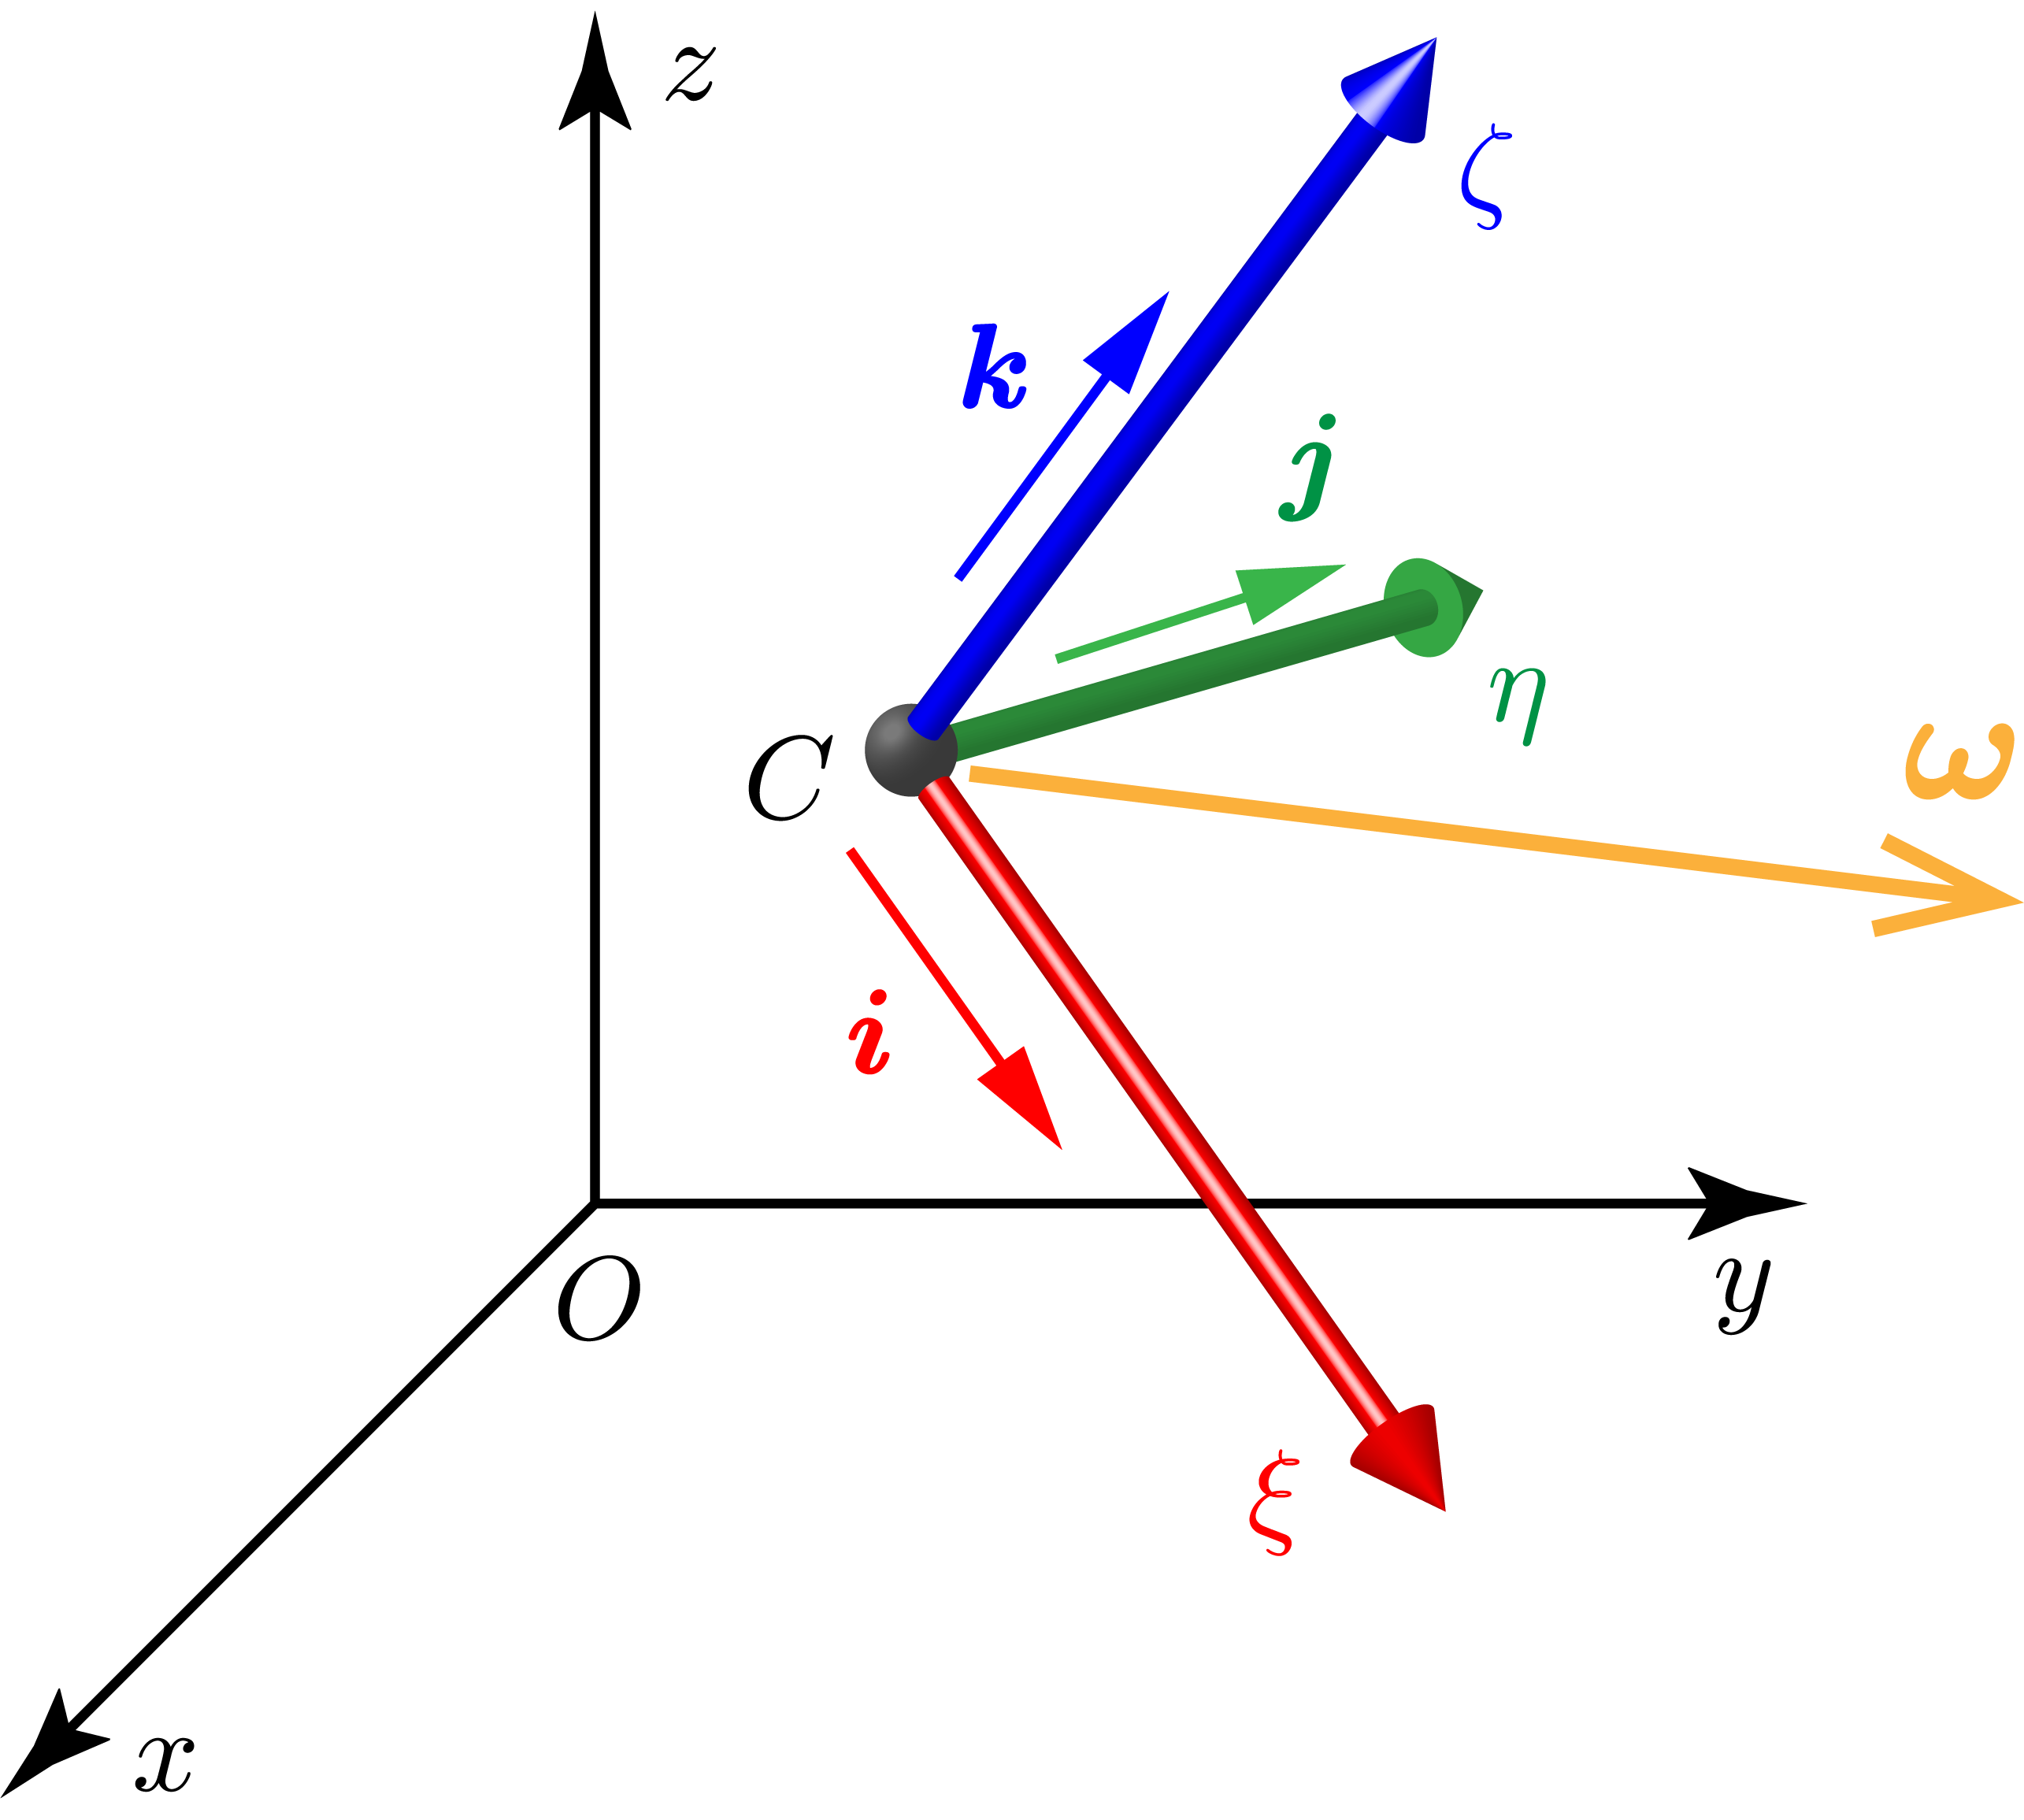
\includegraphics[width=6cm]{image/6-1-8.png}
\caption{刚体的本征框架}
\end{wrapfigure}
为此我们换一种更加直观的方式引入这些概念而不是去严格定义刚体与参考系的概念.\,设想我们有一个正交的刚性框架,\,即三条射线状坐标轴构成的物体,\,下称$\xi,\,\eta,\,\zeta$轴,\,该框架就会自然造成四个矢量.\,首先是框架原点$C$的位置矢量$\bs{r}$.\,其次是三坐标轴方向的三个基矢\footnote{原来的基矢方向记做$\bs{e}_{x,\,y,\,z}$.}$\bs{i},\,\bs{j},\,\bs{k}$.\,它们都会随着时间变化,\,可以用四个导数表征.\,其中$\bs{v}=\dot{\bs{r}},\,\bs{a}=\ddot{\bs{r}}$.\,但是,\,对于三个基矢导数有没有更加简单的描述方法呢?\,如果我们把三个基矢导数就向三个基矢本来的方向分解\footnote{由于字母$i,\,j$上本来就有点,\,所以在符号上约定遇到要在这两个字母上加点时改为横向$\ddot{\imath},\,\ddot{\jmath}$.\,偶尔也见到反而去掉点的$\imath,\,\jmath$.\,出于这样无法表示高阶导数,\,我们不采用这种模式.}:
\[\begin{array}{rlll}
\bs{\ddot{\imath}}=		&	+\omega_{11}\bs{i} 	&	+\omega_{12}\bs{j} 		& +\omega_{13}\bs{k}\\
\bs{\ddot{\jmath}}=		&	+\omega_{21}\bs{i} 	&	+\omega_{22}\bs{j} 		& +\omega_{23}\bs{k}\\
\bs{\dot{k}}=				&	+\omega_{31}\bs{i} 	&	+\omega_{32}\bs{j} 		& +\omega_{33}\bs{k}
\end{array}\]

依然,\,我们注意到出于以下正交归一的结构不会改变,\,在求导下为零,\,所以上述表达式中的九个系数反对称:
\[\frac{\ud}{\ud t}\left\{\begin{array}{cccc}
1= 	&\bs{i}\cdot\bs{i} 	&\bs{j}\cdot\bs{j} 	&\bs{k}\cdot\bs{k} 	\\
0= 	&\bs{i}\cdot\bs{j} 	&\bs{j}\cdot\bs{k} 	&\bs{k}\cdot\bs{i}
\end{array}\right\}=0\quad \Rightarrow \quad\omega_{ij}+\omega_{ji}=0\]

出于某种符号约定与对称的原因,\,我们把导数重新写作:
\[\begin{array}{rlll}
\bs{\ddot{\imath}}=		&									 	&	+\omega_3\bs{j} 				& -\omega_2\bs{k}\\
\bs{\ddot{\jmath}}=		&	-\omega_3\bs{i} 			&									 		& +\omega_1\bs{k}\\
\bs{\dot{k}}=				&	+\omega_2\bs{i} 			&	-\omega_1\bs{j} 				& 
\end{array}\]

这样,\,如果我们定义一个矢量:
\[\bs{\omega}=\omega_1\bs{i}+\omega_2\bs{j}+\omega_3\bs{k}\]

就能够造成:
\[\bs{\ddot{\imath}}=\bs{\omega}\times \bs{i}\quad ,\quad \bs{\ddot{\jmath}}=\bs{\omega}\times \bs{j}\quad ,\quad \bs{\dot{k}}=\bs{\omega}\times \bs{k}\]

这就是刚体的\emph{角速度}(angular velocity)矢量.\,用它可以计算刚体中的各种转动的物理量.

具体来说,\,什么叫做刚体?\,事实上以上三个坐标轴本身就构成了刚体,\,或者是某刚体的一部分.\,如果有一个空间点每时每刻向杆坐标系的三个坐标面引三垂线,\,三个坐标都始终保持常数,\,那么就说这个空间点是\emph{固连}(fixed)在该坐标系中的.\,而如果一个物体上的每一个点都固连带该坐标系中,\,那么相对这个坐标系该物体就无法发生形变,\,从而这就是一个刚体.\,这种情况下,\,刚体与坐标系就存在一个相互关系,\,这个坐标系是由刚体所对应的固连坐标系,\,而坐标系本身又可以视作某种不能变形的刚体.

我们在坐标系中找到固连在坐标系上的两个点,\,或者说在刚体上找到固连在刚体上的两个点(以后不加以区分).\,从一个点指向另一个点形成矢量$\bs{R}$,\,由于固连在坐标系中,\,这个矢量对坐标系造成的三个分量都是固定的,\,也就是$\bs{R}=R_1\bs{i}+R_2\bs{j}+R_3\bs{k}$中的$R_1,\,R_2,\,R_3$都是常数.\,那么这个矢量跟随坐标系而变化的导数就是:
\[\dot{\bs{R}}=R_1\bs{\ddot{\imath}}+R_2\bs{\ddot{\jmath}}+R_3\bs{\dot{k}}=\bs{\omega}\times(R_1\bs{i}+R_2\bs{j}+R_3\bs{k})=\bs{\omega}\times\bs{R}\]

在物理上,\,这就是说,\,任何固连在转动坐标系中的矢量$\bs{R}$都将以角速度$\bs{\omega}$跟随坐标系旋转,\,$\bs{\omega}$的方向就是瞬时转动轴,\,$\bs{\omega}$的大小就是旋转角速度大小.\,注意两点,\,一是这个角速度$\bs{\omega}$是全局的,\,无论矢量相对坐标系在任何位置,\,无论距离最初选取的坐标系中心有多远,\,只要固连在坐标系中,\,就会以完全一样的角速度矢量$\bs{\omega}$去改变$\dot{\bs{R}}=\bs{\omega}\times\bs{R}$.\,二是这个角速度作用在任何量纲上.\,无论是两个空间点之间的那个(位移)矢量,\,还是速度矢量,\,力矢量等等,\,任意量纲的矢量$\bs{A}$只要相对旋转坐标系具有固定的方向,\,在地面系中就会跟着坐标系一同旋转而具有导数:
\[\dot{\bs{A}}=\bs{\omega}\times\bs{A}\quad \text{for }\; \bs{A}\;\text{fixed in frame}\; C-\xi\eta\zeta\]

以后我们可以脱离坐标系而讨论刚体.\,为了研究刚体的运动,\,我们只需要在刚体上取一个合适的固连点$C$作为中心(类似于坐标系的原点),\,这个点叫做\emph{基点}(cardinal point).\,那么,\,不失一般性地,\,刚体的运动将用基点$C$的位置$\bs{r}(t)$和角速度$\bs{\omega}(t)$描述.\,譬如,\,为了求得某一时刻刚体上一点$P$的速度.\,我们可以找到从$C$指向$P$的矢量$\bs{R}$.\,那么,\,由于$\bs{r}_{OC}+\bs{r}_{CP}=\bs{r}_{OP}$.\,这就是说:
\[\bs{v}_{P}=\dot{\bs{r}}_{OP}=\dot{\bs{r}}_{OC}+\dot{\bs{r}}_{CP}=\bs{v}_{C}+\dot{\bs{R}}\]

最后再由之前的用角速度算导数的方法,\,得到著名的基点法速度表达式:
\[\bs{v}_{P}=\bs{v}_{C}+\bs{\omega}\times\bs{R}\]

即:\,刚体上一点速度等于跟随基点平动的速度$\bs{v}_{C}$加上绕基点以$\bs{\omega}$转动的速度$\bs{\omega}\times\bs{R}$的和.

至于加速度,\,只需要对上式再求一次导数$\dot{\bs{v}}_{P}=\dot{\bs{v}}_{C}+\dot{\bs{\omega}}\times\bs{R}+\bs{\omega}\times\dot{\bs{R}}$:
\[\bs{a}_{P}=\bs{a}_{C}+\bs{\beta}\times\bs{R}+\bs{\omega}\times(\bs{\omega}\times\bs{R})\]

即:\,刚体上一点速度等于跟随基点平动的加速度$\bs{a}_{C}$加上绕基点以$\bs{\beta}$转动的角向加速度$\bs{\beta}\times\bs{R}$,\,最后再加上由于速度$\bs{\omega}\times\bs{R}$本身也在绕轴以$\bs{\omega}$旋转带来的向轴加速度$\bs{\omega}\times(\bs{\omega}\times\bs{R})$的和.


\section{参考系变换}

\subsection{点变换}

事实上,\,对旋转坐标系的分析正如对刚体的分析那样,\,一个旋转坐标系的描述正由两点构成,\,一是这个参考系原点$C$的运动方程.\,给出它我们就可以求出任意时刻另一个参考原点的速度与加速度:
\[\bs{v}_C=\dot{\bs{r}}_C\quad,\quad \bs{a}_C=\ddot{\bs{r}}_C\]


\begin{wrapfigure}[14]{o}[-10pt]{6cm}\label{6-1-10}
\vspace{-0.2cm}
\centering
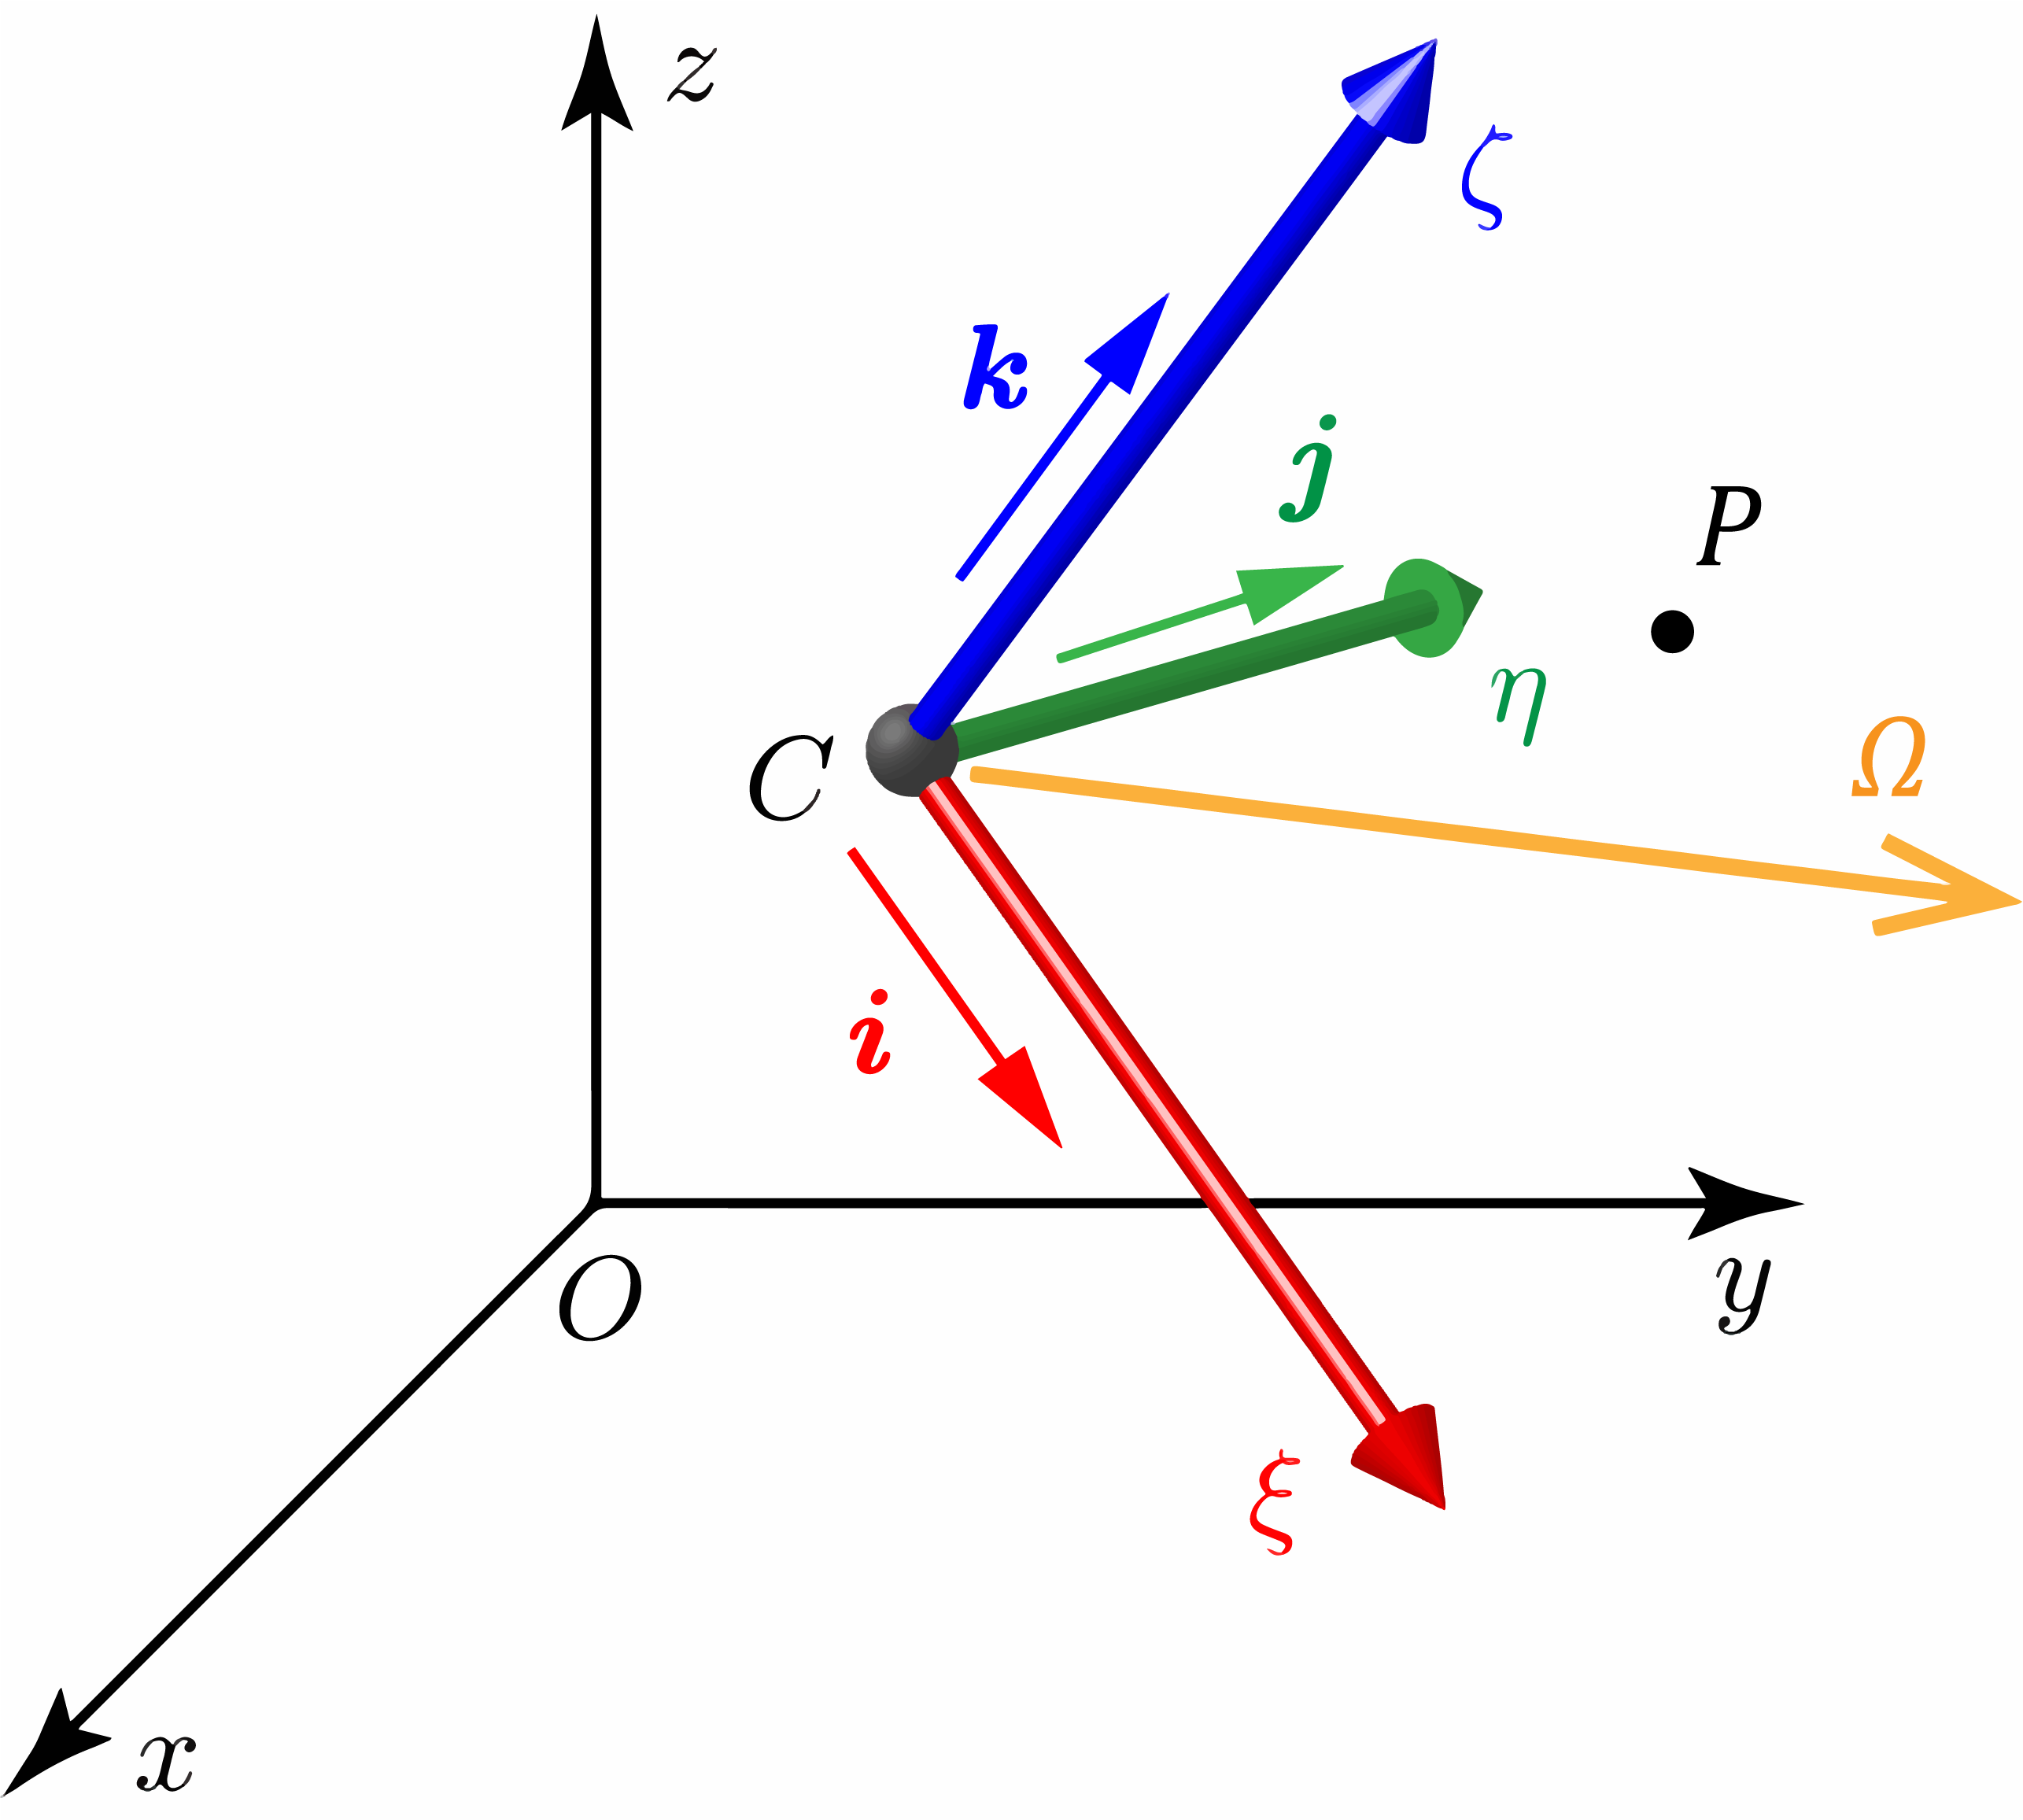
\includegraphics[width=6cm]{image/6-1-10.png}
\caption{参考系变换}
\end{wrapfigure}
第二点就是要给出新参考系的旋转角速度$\bs{\omega}$,\,角加速度记作$\bs{\beta}=\dot{\bs{\omega}}$.\,通过上一节我们知道,\,如果选取固连在新参考系的点$P$,\,并且把$\bs{CP}$记作$\bs{r}'$.\,那么$P$点速度加速度(现在记作$\bs{v}_c,\,\bs{a}_c$)为:
\[\bs{v}_c=\bs{v}_C+\bs{\omega}\times \bs{r}'\]
\[\bs{a}_c=\bs{a}_C+\bs{\omega}\times (\bs{\omega}\times\bs{r}')+\bs{\beta}\times\bs{r}'\]

我们现在研究什么问题呢?\,如果我们在$O-xyz$系中给出一个质点,\,也用$P$表示,\,的运动方程$x(t),\,y(t),\,z(t)$.\,其实也就给出了在$C-\xi\eta\zeta$系中的运动方程$\xi(t),\,\eta(t),\,\zeta(t)$.\,那么把位矢$\bs{OP}$记作$\bs{r}$,\,$\bs{CP}$记作$\bs{r}'$.\,再把$\bs{OC}$记作$\bs{r}_C$.\,于是得到恒等式:
\[\bs{r}=\bs{r}_C+\bs{r}'\]

但这不代表$\bs{v}=\bs{v}_C+\bs{v}'$.\,这里我们要注意有一点已经悄悄发生改变了,\,那就是导数,\,作为一个算符,\,变成了一个有多种自由定义余地的概念.\,只要想想这一点:\,从运动方程求出速度的过程叫做求导\footnote{导数就是从运动方程到速度矢量的映射},\,但是同一个运动方程对应的运动是同一个运动,\,但是在不同参考系中依然可以有多个不同的取值.\,这就足以说明有多种不同的求导方法.\,具体来说,\,这里的$\bs{r}'$可能有三种情况:\,a.\,固连在$C$系中,\,相对$C$系大小方向不变.\,b.\,相对地面系$O$系大小方向都不变,\,即$P$跟随$C$相对地面系平移.\,c.\,两者都不是.\,那么相应地定义三种导数:
\begin{enumerate}
	\item 绝对导数:\,即平常的$\displaystyle\frac{\ud}{\ud t}$,\,可以简单地用加点来代替.\,我们还创造一个新的符号$\uD$来表示求导,\,例如对于情形$b$,\,这个导数就是零.\,求导数的方法是:\,找到一个矢量在$O$系中每时每刻向三个坐标轴方向的投影分量并分别求导最后组合为矢量.\,用这个导数能定义$P$点在$O$系中的速度与加速度:
	\[\bs{v}=\uD \bs{r}(=\frac{\ud}{\ud t}\bs{r}=\dot{\bs{r}})\quad,\quad\bs{a}=\uD \bs{v} \]
	\item 相对导数:\,这就是要换相对$C$系的视角来研究一个矢量的导数了.\,我们记作$\uD'$.\,例如对于情形$a$,\,那么相对导数就是零.\,求导数的方法是:\,找到一个矢量在$C$系中每时每刻向三个坐标轴方向的投影分量并分别求导最后组合为矢量.\,这也就是说它用来定义相对速度和相对加速度是合适的:
	\[\bs{v}'=\uD'\bs{r}'=\dot{r_1'}\bs{i}+\dot{r_2'}\bs{j}+\dot{r_3'}\bs{k}\quad ,\quad \bs{a}'=\uD'\bs{v}'=\ddot{r_1'}\bs{i}+\ddot{r_2'}\bs{j}+\ddot{r_3'}\bs{k}\]
	\item 随体导数:\,这是矢量由于跟随$C$系转动而带来的相对$O$系的变化率.\,我们记作$\widetilde{\uD}$.\,例如在情形$a$中,\,$\bs{r}'$随体导数就是$\bs{\omega}\times\bs{r}'$.\,这个算符其实就等价于$\omega\times$,\,这是因为他就定义为:
	\[\widetilde{\uD}\bs{A}=A_1\bs{\ddot{\imath}}+A_2\bs{\ddot{\jmath}}+A_3\bs{\dot{k}}=A_1\bs{\omega}\times\bs{i}+A_2\bs{\omega}\times\bs{j
	}+A_3\bs{\omega}\times\bs{k}=\bs{\omega}\times(A_1\bs{i}+A_2\bs{j}+A_3\bs{k})=\bs{\omega}\times\bs{A}\]
\end{enumerate}

值得注意的是,\,这三个导数算符之间有如下关系:
\[\uD=\widetilde{\uD}+\uD'\]

这很容易证明,\,对一个矢量求导数,\,一看分量变不变,\,而看基矢量本身有没有旋转.\,那么就会产生两项.\,实际上就是莱布尼茨法则.

于是这才能推理参考系变换的公式.\,我们对$\bs{r}=\bs{r}_C+\bs{r}'$两边求绝对导数:
\[\bs{v}=\uD\bs{r}=\uD\bs{r}_C+\uD\bs{r}'=\bs{v}_C+(\widetilde{\uD}+\uD')\bs{r}'=\bs{v}_C+\bs{\omega}\times\bs{r}'+\bs{v}'\]

再次对上式两边求绝对导数:
\begin{align*}
\bs{a}=\uD\bs{v} &=\uD\bs{v}_C+\uD\bs{\omega}\times\bs{r}'+\bs{\omega}\times\uD\bs{r}'+\uD\bs{v}'\\
	  			 &=\bs{a}_C+\bs{\beta}\times\bs{r}'+\bs{\omega}\times(\widetilde{\uD}+\uD')\bs{r}'+(\widetilde{\uD}+\uD')\bs{v}'\\
	  			 &=\bs{a}_C+\bs{\beta}\times\bs{r}'+\bs{\omega}\times(\bs{\omega}\times\bs{r}')+\bs{\omega}\times\bs{v}'+\bs{\omega}\times\bs{v}'+\bs{a}'\\
	  			 &=\bs{a}_C+\bs{\beta}\times\bs{r}'+\bs{\omega}\times(\bs{\omega}\times\bs{r}')+2\bs{\omega}\times\bs{v}'+\bs{a}'
\end{align*}

这两个公式就是参考系变换下的变换公式:
\[\bs{v}=\bs{v}_C+\bs{\omega}\times\bs{r}'+\bs{v}'\]
\[\bs{a}=\bs{a}_C+\bs{\beta}\times\bs{r}'+\bs{\omega}\times(\bs{\omega}\times\bs{r}')+2\bs{\omega}\times\bs{v}'+\bs{a}'\]

如何理解以上的公式?\,事实上结构也很简单,\,我们把加速度中的最独特的一项单独拿出来叫做\emph{柯里奥利加速度}(Coriolis accelaration):
\[a_c'=2\bs{\omega}\times\bs{v}'\]

那么以上两公式具有以下结构:
\[\text{绝对}=\text{牵连}(+\text{柯氏})+\text{相对}\]

柯氏即柯里奥利.\,相对速度与相对加速度就是$\bs{v}',\,\bs{a}'$.\,言下之意就是我们定义了所谓的\emph{牵连速度}(convected velocity)与\emph{牵连加速度}(convected acceleration):
\[\bs{v}_c=\bs{v}_C+\bs{\omega}\times \bs{r}'\]
\[\bs{a}_c=\bs{a}_C+\bs{\omega}\times (\bs{\omega}\times\bs{r}')+\bs{\beta}\times\bs{r}'\]

细心的读者已经发现了,\,这两个式子和本节最开始推导出来的固连在$C$系中的点的绝对速度,\,加速度公式是一致的.\,牵连速度(加速度),\,顾名思义,\,被转动参考系``带着走''的速度(加速度).\,也正是以上规律启发我们总结出以下的动点动系法来理解看似复杂的速度加速度合成公式:
\begin{enumerate}
	\item 确定定系,\,动系,\,动点,\,定点.\,定系往往就是地面系;\,动系一般是相对某刚体或人为构造的刚性框架相对静止的参考系\footnote{注意,\,以下整个过程都可以脱离具体的坐标系而计算,\,这就为坐标系的选取(种类是直角坐标系,\,极座标系还是自然坐标系,\,方向如何)彻底提供了自由.};\,动点就是选做研究对象的相对两个系一般都有运动的点.\,最后,\,定点指的是这样的概念:\,在研究的一瞬间与动点重合,\,但是始终保持与动系固连的特殊参考点.
	\item 在定系考虑动点的运动.\,算出绝对量.\,在动系考虑动点的运动.\,算出相对量.\,在定系中考虑定点的运动,\,它的量就是牵连量.
	\item 建立绝对相对牵连之间的等量关系.
	\item 唯一要注意的是:\,只有当转动系是真转动的$\bs{\omega}\neq\bs{0}$,\,而且相对动系动点也是真运动的$\bs{v}'\neq\bs{0}$时,\,我们才有必要在加速度中添加一项柯氏加速度$2\bs{\omega}\times\bs{v}'$.\,从推导过程来看,\,一是即使固连在动系中的速度矢量也会跟随动系转动而带来加速度,\,二是动系中的相对位矢产生变化而带来在变化的牵连速度从而产生加速度,\,是造成柯氏加速度的两个因素.\,这一项不是因为在动系中的某特定位置而造成的,\,事实上与$\bs{r}'$无关,\,决定性因素是``相对动系有速度''.
\end{enumerate}

最后值得注意,\,如果$\bs{\omega}$和$\bs{\beta}$恒为零,\,这也并不少见,\,那么这样的动系就是\emph{平动系}(translational frame).\,此时公式极为简单,\,没有柯氏加速度,\,牵连量就是动系原点或任意固连点的量:
\[\bs{v}=\bs{v}_C+\bs{v}'\quad,\quad \bs{a}=\bs{a}_C+\bs{a}'\]

\subsection{刚体变换}

刚体的变换是点变换的直接推论.\,同样地,\,首先已知动系相对定系具有原点速度$\bs{v}_C$和加速度$\bs{a}_C$以及角速度$\bs{\omega}$和加速度$\bs{\beta}$,\,又已知定系中刚体基点速度加速度,\,现在记作$\bs{V},\,\bs{A}$.\,事实上我们还要给出刚体自己的角速度角加速度才算是对刚体的完整描述,\,它们为$\bs{\varOmega},\,\bs{B}$.\,那么绝对的和相对的各个量之间的关系为:
\[\bs{V}=\bs{v}_C+\bs{\omega}\times\bs{R}'+\bs{V}'\quad,\quad \bs{\varOmega}=\bs{\omega}+\bs{\varOmega}'\]
\[\bs{A}=\bs{a}_C+\bs{\beta}\times\bs{R}'+\bs{\omega}\times(\bs{\omega}\times\bs{R}')+2\bs{\omega}\times\bs{V}'+\bs{A}'\quad,\quad \bs{B}=\bs{\beta}+\omega\times\bs{\varOmega}'+\bs{B}'\]

证明过程留作练习由读者自己思考.

\section{运动的牵连}
最后本节旨在枚举一些在运动学解题中十分常见的初等模型与结论.

\subsection{接触系}
两个几何图形具有一个交点是一件非常常见的事情.\,交点将同时与两个几何图形保持结合关系.\,动态地看待这个问题,\,我们可以分别利用两个几何图形自身的运动和交点相对两者的运动合成来写出交点的速度矢量与加速度矢量来,\,但是作为同一个研究对象两种写法的结果理应相等.\,这构成了一组方程.

尤其是,\,在上述``相交系''中我们还有一类十分独特的情形,\,就是两个几何图形相切.\,两个平面形刚体如果始终保持相互接触,\,其轮廓之间就是这样的关系.\,此时要知道客观地这形除了一种约束:\,不是让两个刚体做任意运动都可以让两者保持相切的.\,所以必然存在所谓的\emph{约束方程}(equation of constraint).\,而这个方程的列法其实就是基于之前说的接触点的速度的一致性.

让我们看一个例子,\,它不仅帮助我们理解接触系,\,还可以帮助我们理解纯滚系.\,就是经典的在粗糙的地面上做匀速纯滚动的圆盘.\,首先应当注意到,\,涉及到所谓的``瞬时接触点''时可能指的是以下三个点之一:
\begin{wrapfigure}[8]{o}[-10pt]{7cm}
\vspace{0.1cm}
\centering
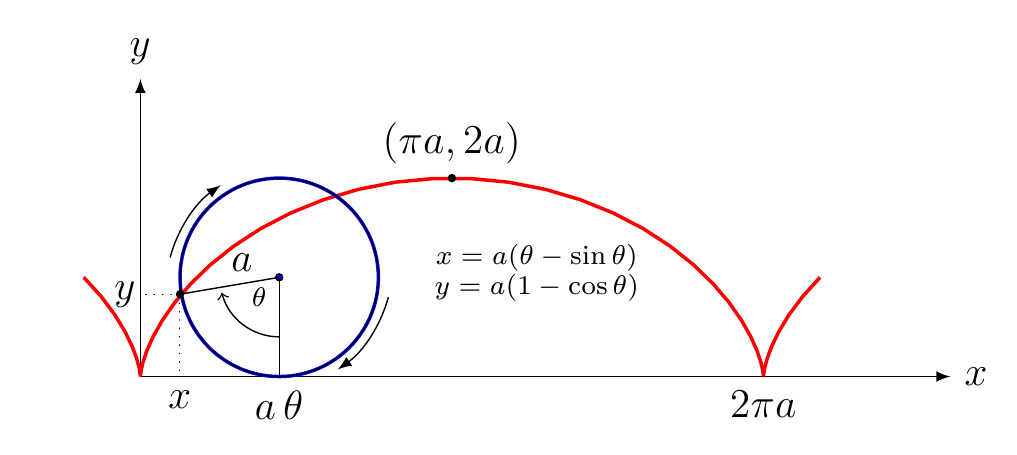
\includegraphics[width=7cm]{image/6-1-11.png}
\caption{圆盘在地面上做纯滚动}
\end{wrapfigure}

1.\,刚体1上的定点$P_1$.\,在这里取盘为刚体1,\,此时这个点是做旋轮线运动的那个点,\,此时恰好位于最低位置.

2.\,刚体2上的定点$P_2$.\,在这里取地面为刚体2,\,那么这个点就是一个静止的点.

3.\,动点$P_3$.\,就是每时每刻的切点形成的运动对象.\,在这里我们可以把圆盘变为圆筒,\,并且让一只松鼠在圆筒内部跑动以保持在最低位置,\,也就是每时每刻的切点.\,那么松鼠做匀速直线运动.

我们有什么结论呢?\,如果把$P_1$的瞬时速度在法线方向与切线方向的分速度与加速度写出来,\,分别是$v_{1n},\,v_{1\tau},\,a_{1n},\,a_{1\tau}$并约定法向以向刚体1内侧为正,\,切向可以以切线的任意一个方向为正.\,$P_2$同理为$v_{2n},\,v_{2\tau},\,a_{2n},\,a_{2\tau}$.\,那么让我们考虑一下$P_3$的速度与加速度.\,这就不难发现,\,如果采用动点动系法,\,就有:

速度:\,无论相对刚体1还是2,\,$P_3$的速度都是牵连加相对.\,牵连速度就是定点的速度,\,但相对速度由于点的轨迹就是刚体的轮廓,\,故方向必然在切线方向.\,然后由于速度的唯一性,\,这可以给出:
\[v_{1n}=-v_{2n}\]

加速度:\,道理是相同的,\,但需要注意两点,\,一是相对加速度具有了法线方向的分量.\,二是如果严格换一个刚体的转动系往往会带来柯氏加速度.\,具体解题时这仍然不失为一种常见的解题思路,\,但是难以总结现成的美妙,\,下一小节通过添加纯滚动这一更强的结论我们可以得到相应的方程.\,但是这个方程肯定是存在且可列式的,\,毕竟:

以上两个方程构成对接触系的约束的刻画.

\subsection{纯滚系}
上面的圆盘在地面上发生的运动实际上还是纯滚动.\,我们将首先给出纯滚动的定义,\,再来讨论纯滚动时的更强的附加条件,\,毕竟纯滚动相比简单的接触系还多一个约束.

事实上考虑相对运动就知道了,\,接触点在刚体1或2上相对运动的弧长就是相互滚动过的接触弧长,\,在两个刚体上应当具有公共值,\,这便是纯滚动的定义.\,这就是说:
\[\bs{v}_1'=\bs{v}_2'=\dot{s}\bs{\tau}\]

最后再利用$\bs{v}=\bs{v}_{1c}+\bs{v}_1'=\bs{v}_{2c}+\bs{v}_2'$.\,便得到了附加条件:
\[v_{1\tau}=v_{2\tau}\]

这就是常见的纯滚条件一,\,也就是说只有当相互接触的两个刚体定点切向速度一致才构成纯滚动.\,否则就是纯滚动的反面:\,必有相对滑动,\,俗称``连滚带滑''.

考虑加速度我们将得出一个不可思议但容易忽视的结论.\,首先注意到,\,如果两个刚体角速度分别为$\omega_1$和$\omega_2$,\,作为平面问题写成统一正方向的标量.\,而再设两刚体在接触点处轮廓的曲率为$k_1$和$k_2$.\,那么由于相对两刚体点在轮廓上的运动造成的单位时间切线方向的转角为:
\[\frac{\ud\theta_1}{\ud t}=\frac{\ud\theta_1}{\ud s}\frac{\ud s}{\ud t}=k_1\dot{s}\]
\[\frac{\ud\theta_2}{\ud t}=\frac{\ud\theta_2}{\ud s}\frac{\ud s}{\ud t}=k_2\dot{s}\]

而每当点成为切点两切线也会重合成为公切线,\,那么两个转角的和就是单位时间内两个刚体的相对转角:
\[\frac{\ud\theta_1}{\ud t}+\frac{\ud\theta_2}{\ud t}=|\omega_1-\omega_2|\]

最后,\,列出对刚体1和2牵连+柯氏+相对应当一致的方程:
\[a_{1n}-2\omega_1 \dot{s}+k_1\dot{s}^2=-(a_{2n}-2\omega_2\dot{s}+k_2\dot{s}^2)\]

整理得到纯滚条件二:
\[a_{1n}+a_{2n}=\frac{(\omega_1-\omega_2)^2}{k_1+k_2}\]

这是一个必然大于零的表达式\footnote{注意$k$本身可以小于零,\,但两个$k$的和必然大于零.},\,它意在,\,两个相接触的点必然后来会分离,\,这个分离加速度只与两刚体瞬时转动快慢和接触点弯曲程度有关,\,与平动转动加速度都没有关系.

\subsection{约束系}
约束是一种普遍存在且可以普遍讨论而有很广的适用范围的物理现象.\,本节并非要详细讨论约束,\,这一点在之后第三章静力学中再加以详细讨论.\,这里只讨论两个问题:\,绳系和杆系.

对于不可伸长的轻绳模型,\,如果它也被拉直(因为内部受力不为零又没有外力).\,那么在运动学层面上就等价于不可伸长的轻杆.\,设杆长为$l$,\,把两端点1和2速度加速度沿平行与杆与垂直与杆方向分解,\,具有关系:
\[v_{1\perp}-v_{2\perp}=\omega l\]
\[v_{1\parallel}-v_{2\parallel}=0\]
\[a_{1\perp}-a_{2\perp}=\beta l\]
\[a_{1\parallel}-a_{2\parallel}=-\omega^2 l\]

其中第二个关系就是著名的端点沿杆方向分速度必须是常数.\,对于绳子,\,即使绕过了定滑轮,\,显然沿定滑轮的切向速度也一直不变,\,因为绳子不可伸长.

最后,\,如果绳子允许弯曲但不允许伸长,\,其运动学约束方程该如何列?\,那就要求绳子上每一点在``局部''沿切向方向没有相对速度,\,表示为公式就是:
\[\frac{\ud \bs{v}}{\ud s}\cdot\bs{\tau}=0\]

注意这个条件不可以写为:
\[\frac{\ud v_\tau}{\ud s}=\frac{\ud (\bs{v}\cdot\bs{\tau})}{\ud s}=0\]
